% ============================================================================
% Rapport de Stage de Fin d'Année — EMSI, filière DSIC (Groupe G3)
% Plateforme de notifications omnicanales et de workflows pilotée par événements
% 6Solutions — Saad DINARI & Saad HARRAGUI
%
% Note de transcription : les icônes/émojis décoratifs visibles dans
% l'interface réelle (⚡, 🔄, ●, 📤, etc.) ont été omis dans ce document
% LaTeX afin de garantir une compilation propre avec le moteur pdfLaTeX et
% l'encodage utf8 classique (inputenc). Les libellés textuels des boutons et
% badges de l'interface sont en revanche restitués fidèlement entre
% guillemets.
% ============================================================================

\documentclass[12pt,a4paper]{report}

% ───────────────────────────── Encodage et langue ─────────────────────────────
\usepackage[utf8]{inputenc}
\usepackage[T1]{fontenc}
\usepackage[french]{babel}
\usepackage{lmodern}
\usepackage{microtype}

% ───────────────────────────── Mise en page ─────────────────────────────
\usepackage[a4paper,left=3cm,right=2.5cm,top=2.5cm,bottom=2.5cm,headheight=15pt]{geometry}
\usepackage{setspace}
\onehalfspacing
\setlength{\parindent}{1cm}
\setlength{\parskip}{4pt}

% ───────────────────────────── Couleurs ─────────────────────────────
\usepackage[table]{xcolor}
\definecolor{darkblue}{HTML}{1F3864}
\definecolor{midblue}{HTML}{2E4C7E}
\definecolor{placeholderred}{HTML}{C00000}
\definecolor{greytext}{HTML}{808080}

% ───────────────────────────── Tableaux, figures ─────────────────────────────
\usepackage{graphicx}
\usepackage{float}
\usepackage{longtable}
\usepackage{array}
\usepackage{ragged2e}
\usepackage{caption}
% babel re-applies its own caption strings every time French is (re)selected,
% so this is redefined right after \begin{document} AND right after the one
% \selectlanguage{french} switch-back (see Abstract section below), rather
% than relying on babel's internal per-language macro names.
\newcommand{\fixfrenchcaptions}{%
  \renewcommand{\figurename}{Figure}%
  \renewcommand{\tablename}{Tableau}%
}
\captionsetup{font={bf,it,small},labelsep=colon,justification=centering}
\captionsetup[longtable]{font={bf,it,small},labelsep=colon}

% ───────────────────────────── Listes ─────────────────────────────
\usepackage{enumitem}
\setlist[itemize]{leftmargin=1.2cm, itemsep=4pt, topsep=4pt}

% ───────────────────────────── Titres de chapitres/sections ─────────────────────────────
\usepackage{titlesec}

\titleformat{\chapter}[display]
  {\normalfont}
  {\color{greytext}\Large\MakeUppercase{\chaptertitlename}~\thechapter}
  {8pt}
  {\color{darkblue}\Huge\bfseries}
  [\vspace{4pt}{\color{darkblue}\titlerule[1.2pt]}\vspace{10pt}]
\titlespacing*{\chapter}{0pt}{10pt}{20pt}

\titleformat{\section}
  {\normalfont\Large\bfseries\color{darkblue}}{\thesection}{0.6em}{}
\titlespacing*{\section}{0pt}{16pt}{8pt}

\titleformat{\subsection}
  {\normalfont\large\bfseries\color{midblue}}{\thesubsection}{0.6em}{}
\titlespacing*{\subsection}{0pt}{12pt}{6pt}

\setcounter{secnumdepth}{2}
\setcounter{tocdepth}{2}

% ───────────────────────────── En-tête / pied de page ─────────────────────────────
\usepackage{fancyhdr}
\pagestyle{fancy}
\fancyhf{}
\renewcommand{\headrulewidth}{0.4pt}
\fancyhead[R]{\textit{\textcolor{greytext}{Rapport de Stage de Fin d'Année --- 6Solutions}}}
\fancyfoot[C]{\thepage}
\fancypagestyle{plain}{%
  \fancyhf{}
  \fancyfoot[C]{\thepage}
  \renewcommand{\headrulewidth}{0pt}
}

% ───────────────────────────── Liens (hyperref, en dernier) ─────────────────────────────
\usepackage{hyperref}
\hypersetup{
  colorlinks=true,
  linkcolor=darkblue,
  citecolor=darkblue,
  urlcolor=darkblue,
  pdftitle={Rapport de Stage de Fin d'Année --- Plateforme de notifications omnicanales et de workflows pilotée par événements},
  pdfauthor={Saad DINARI et Saad HARRAGUI},
  pdfsubject={Rapport de Stage de Fin d'Année - EMSI - DSIC},
}

% ───────────────────────────── Commande pour les placeholders ─────────────────────────────
\newcommand{\placeholder}[1]{\par\smallskip\noindent\textcolor{placeholderred}{\itshape [#1]}\par\smallskip}

% ============================================================================
\begin{document}
\fixfrenchcaptions

% ---------------------------------------------------------------------------
% Page de garde
% ---------------------------------------------------------------------------
\begin{titlepage}
\thispagestyle{empty}
\centering
\vspace*{0.3cm}
{\bfseries\large ÉCOLE MAROCAINE DES SCIENCES DE L'INGÉNIEUR}\\[0.2cm]
{\bfseries (EMSI)}\\[0.2cm]
Cycle Ingénieur --- Filière DSIC (Groupe G3)\\[0.8cm]

\placeholder{Emplacement réservé au logo officiel de l'EMSI}

\vspace{1cm}
{\bfseries\Huge Rapport de Stage de Fin d'Année}\\[0.6cm]
pour l'obtention du\\[0.2cm]
{\bfseries\large Diplôme d'Ingénieur d'État}\\[0.6cm]
{\bfseries Filière : Génie Informatique --- DSIC (Groupe G3)}\\[1.2cm]

Présenté par :\\[0.2cm]
{\bfseries\large Saad DINARI \quad \& \quad Saad HARRAGUI}\\[1.2cm]

\noindent\rule{\linewidth}{0.6pt}\\[0.35cm]
{\bfseries\Large Plateforme de notifications omnicanales et de workflows pilotée par événements}\\[0.35cm]
\noindent\rule{\linewidth}{0.6pt}\\[1.2cm]

Stage effectué au sein de :\\[0.3cm]

\includegraphics[width=4.5cm]{figures/6solutions-logo.png}\\[0.3cm]
{\itshape Consulting.Technology}\\[1.2cm]

Encadrant académique (EMSI) : \textcolor{placeholderred}{\itshape [Nom de l'encadrant académique]}\\[0.25cm]
Encadrant professionnel (6Solutions) : \textcolor{placeholderred}{\itshape [Nom de l'encadrant professionnel]}\\[1.2cm]

{\bfseries Année universitaire : }\textcolor{placeholderred}{\itshape [À préciser]}
\vfill
\end{titlepage}

% ---------------------------------------------------------------------------
% Pagination romaine pour le préambule
% ---------------------------------------------------------------------------
\pagenumbering{roman}

% ---------------------------------------------------------------------------
% Dédicace
% ---------------------------------------------------------------------------
\chapter*{Dédicace}
\addcontentsline{toc}{chapter}{Dédicace}

\placeholder{Cette page vous appartient. Traditionnellement, l'étudiant y dédie son travail à ses parents, à sa famille, à ses proches et à toute personne ayant compté durant son parcours. Merci de la rédiger vous-même, dans vos propres mots -- je peux vous proposer une trame si vous le souhaitez, mais ce texte est personnel et ne doit pas être écrit à votre place.}

% ---------------------------------------------------------------------------
% Remerciements
% ---------------------------------------------------------------------------
\chapter*{Remerciements}
\addcontentsline{toc}{chapter}{Remerciements}

Au terme de ce stage de fin d'année, nous tenons à exprimer notre profonde gratitude envers l'ensemble des personnes qui ont contribué, de près ou de loin, à la réussite de ce travail.

Nous adressons tout d'abord nos sincères remerciements au corps professoral et administratif de l'\textbf{École Marocaine des Sciences de l'Ingénieur (EMSI)}, pour la qualité de la formation dispensée tout au long de notre cursus d'ingénieur, filière DSIC.

Nous tenons à remercier tout particulièrement notre encadrant académique, \textcolor{placeholderred}{\itshape [Nom de l'encadrant académique]}, pour ses conseils avisés, sa disponibilité et le suivi rigoureux qu'il/elle nous a accordé tout au long de ce projet.

Nos remerciements s'adressent également à toute l'équipe de \textbf{6Solutions}, et tout particulièrement à notre encadrant professionnel, \textcolor{placeholderred}{\itshape [Nom de l'encadrant professionnel]}, pour son accueil chaleureux, sa disponibilité constante et ses précieux conseils techniques qui nous ont permis de mener ce projet dans les meilleures conditions.

Enfin, nous remercions les membres du jury pour l'intérêt qu'ils ont porté à ce travail en acceptant de l'évaluer, ainsi que toute personne ayant contribué, directement ou indirectement, à l'aboutissement de ce projet.

% ---------------------------------------------------------------------------
% Résumé
% ---------------------------------------------------------------------------
\chapter*{Résumé}
\addcontentsline{toc}{chapter}{Résumé}

\textcolor{placeholderred}{\itshape Brouillon --- à affiner une fois l'ensemble des chapitres rédigés.}

\bigskip

Ce rapport est réalisé dans le cadre du stage de fin d'année pour l'obtention du diplôme d'Ingénieur d'État en Génie Informatique, filière DSIC, à l'École Marocaine des Sciences de l'Ingénieur (EMSI). Il s'est déroulé au sein de la société 6Solutions (Consulting \& Technology) et porte sur la conception et le développement d'une plateforme de notifications omnicanales et de workflows pilotée par événements.

Dans un contexte où les organisations doivent communiquer avec leurs utilisateurs de manière fiable, instantanée et personnalisée à travers de multiples canaux (Email, SMS, Push), ce projet répond au besoin de centraliser l'ingestion des événements métier, d'orchestrer leur traitement via un moteur de workflows configurable, et d'assurer une diffusion omnicanale robuste des notifications, avec gestion des préférences utilisateur, des mécanismes de repli (fallback) et des plages de silence (quiet hours).

La solution repose sur une architecture orientée événements combinant Apache Kafka pour le streaming des événements, un backend Spring Boot (ingestion-service) sécurisé par authentification JWT via Keycloak, et un frontend Angular pour la construction visuelle des workflows, le suivi des exécutions et la simulation d'événements en temps réel. Une attention particulière a été portée à la qualité logicielle : la suite de tests, développée avec JUnit 5, Mockito côté backend et Jasmine/Karma côté frontend, a permis d'atteindre une couverture de code de 87,4~\% sur le backend et de 93,0~\% sur le frontend, vérifiée via SonarQube.

Le projet a été mené selon la méthodologie Agile Scrum, avec un versionnement Git/GitHub et une conteneurisation Docker des différents services.

\medskip
\noindent\textbf{Mots clés :} notifications omnicanales, architecture événementielle, Apache Kafka, moteur de workflows, Spring Boot, Angular, Keycloak, SonarQube, méthodologie Scrum.

% ---------------------------------------------------------------------------
% Abstract
% ---------------------------------------------------------------------------
\chapter*{Abstract}
\addcontentsline{toc}{chapter}{Abstract}
\selectlanguage{english}

\textcolor{placeholderred}{\itshape Draft --- to be refined once every chapter has been written.}

\bigskip

This report was prepared as part of the end-of-year internship for the State Engineer's degree in Computer Engineering, DSIC track, at the École Marocaine des Sciences de l'Ingénieur (EMSI). It was carried out within 6Solutions (Consulting \& Technology) and focuses on the design and development of an event-driven omnichannel notification and workflow platform.

In a context where organizations must communicate with their users reliably, instantly and in a personalized way across multiple channels (Email, SMS, Push), this project addresses the need to centralize the ingestion of business events, orchestrate their processing through a configurable workflow engine, and ensure robust omnichannel delivery of notifications, including user preference management, fallback mechanisms and quiet-hours suppression.

The solution relies on an event-driven architecture combining Apache Kafka for event streaming, a Spring Boot backend (ingestion-service) secured by JWT authentication via Keycloak, and an Angular frontend for visually building workflows, monitoring executions and simulating events in real time. Particular attention was paid to software quality: the test suite, built with JUnit 5 and Mockito on the backend and Jasmine/Karma on the frontend, achieved a code coverage of 87.4\% on the backend and 93.0\% on the frontend, verified through SonarQube.

The project was conducted using the Agile Scrum methodology, with Git/GitHub version control and Docker containerization of the different services.

\medskip
\noindent\textbf{Keywords:} omnichannel notifications, event-driven architecture, Apache Kafka, workflow engine, Spring Boot, Angular, Keycloak, SonarQube, Scrum methodology.

\selectlanguage{french}
\fixfrenchcaptions

% ---------------------------------------------------------------------------
% Table des matières / listes
% ---------------------------------------------------------------------------
\tableofcontents

\listoffigures
\addcontentsline{toc}{chapter}{Table des figures}

\listoftables
\addcontentsline{toc}{chapter}{Liste des tableaux}

% ---------------------------------------------------------------------------
% Liste des sigles et acronymes
% ---------------------------------------------------------------------------
\chapter*{Liste des sigles et acronymes}
\addcontentsline{toc}{chapter}{Liste des sigles et acronymes}

\begin{longtable}{@{}p{0.22\textwidth}p{0.65\textwidth}@{}}
\textbf{API} & Application Programming Interface \\
\textbf{JWT} & JSON Web Token \\
\textbf{REST} & Representational State Transfer \\
\textbf{JSON} & JavaScript Object Notation \\
\textbf{UML} & Unified Modeling Language \\
\textbf{HTTP} & HyperText Transfer Protocol \\
\textbf{IDE} & Integrated Development Environment \\
\textbf{CI/CD} & Continuous Integration / Continuous Delivery \\
\textbf{SGBD} & Système de Gestion de Base de Données \\
\end{longtable}

\textit{\textcolor{greytext}{\small Liste non exhaustive à ce stade : elle sera complétée au fil de la rédaction des chapitres techniques (environnement de développement, architecture, réalisation).}}

% ---------------------------------------------------------------------------
% Pagination arabe pour le corps du rapport
% ---------------------------------------------------------------------------
\clearpage
\pagenumbering{arabic}
\setcounter{page}{1}

% ============================================================================
% Introduction Générale
% ============================================================================
\chapter*{Introduction Générale}
\addcontentsline{toc}{chapter}{Introduction Générale}

La transformation numérique a profondément modifié la manière dont les organisations communiquent avec leurs clients, leurs partenaires et leurs collaborateurs. Aujourd'hui, un système d'information ne se limite plus à traiter et stocker des données : il doit être capable de réagir en temps réel aux événements qui surviennent dans son environnement, et d'en informer les bonnes personnes, au bon moment, par le canal le plus approprié.

Les notifications occupent à ce titre une place centrale dans les systèmes d'information modernes. Qu'il s'agisse de confirmer une opération, d'alerter un utilisateur ou de l'accompagner tout au long d'un parcours, elles constituent le lien direct entre une application et ses utilisateurs. Cette exigence se heurte cependant à plusieurs difficultés récurrentes : la multiplication des canaux de communication (Email, SMS, notifications Push), l'hétérogénéité des règles métier associées à chaque type d'événement, la nécessité de garantir la fiabilité de l'acheminement même en cas d'échec d'un canal, et enfin l'absence fréquente d'un mécanisme centralisé permettant d'orchestrer ces envois de façon cohérente, traçable et évolutive.

Au-delà du simple envoi de messages, de nombreux processus métier gagnent à être automatisés sous forme de workflows déclenchés par des événements : une action doit parfois enclencher une séquence de traitements conditionnels --- attendre un délai, vérifier une condition, notifier un utilisateur, puis clôturer le processus --- sans qu'il soit nécessaire de coder chaque scénario de façon rigide. La possibilité de concevoir, valider et exécuter de tels enchaînements de manière visuelle et configurable représente un enjeu important pour la réactivité et l'agilité des systèmes d'information.

C'est dans ce contexte que s'inscrit le présent projet, mené au sein de la société \textbf{6Solutions}, et consacré à la conception et à la réalisation d'une \textbf{\textit{plateforme de notifications omnicanales et de workflows pilotée par événements}}. Cette plateforme vise à centraliser l'ingestion des événements métier, à orchestrer leur traitement à travers un moteur de workflows configurable, et à garantir une diffusion fiable des notifications sur plusieurs canaux, tout en offrant des outils de suivi, de simulation et de supervision.

La réalisation de ce projet a couvert l'ensemble du cycle de développement logiciel : l'analyse du contexte et des besoins, l'étude des spécifications fonctionnelles et non fonctionnelles, la conception de l'architecture technique, le développement des composants backend et frontend, ainsi que la mise en place d'une démarche de test rigoureuse appuyée par des outils d'analyse de qualité de code.

Ce rapport présente la démarche suivie et les résultats obtenus, organisés selon le plan suivant :

\begin{itemize}
  \item \textbf{Chapitre 1 --- Présentation du cadre du projet :} ce chapitre présente l'organisme d'accueil, 6Solutions, ainsi que le contexte général, la problématique, les objectifs et la méthodologie de travail adoptée pour la réalisation du projet.
  \item \textbf{Chapitre 2 --- Spécification des besoins fonctionnels et non fonctionnels :} ce chapitre détaille les besoins recueillis, les acteurs du système, les cas d'utilisation ainsi que les exigences de qualité attendues de la solution.
  \item \textbf{Chapitre 3 --- Conception et architecture :} ce chapitre présente la modélisation UML du système (diagrammes de cas d'utilisation, de séquence et de classes) ainsi que l'architecture globale, backend et frontend, retenue pour la solution.
  \item \textbf{Chapitre 4 --- Environnement et outils de développement :} ce chapitre décrit les langages, frameworks, outils et technologies mobilisés pour la mise en \oe uvre du projet.
  \item \textbf{Chapitre 5 --- Réalisation, tests et couverture de code :} ce chapitre présente les principales fonctionnalités développées, la stratégie de test mise en \oe uvre ainsi que les résultats de couverture de code obtenus via SonarQube.
\end{itemize}

Le rapport se conclut par une synthèse générale du travail réalisé, un retour d'expérience sur les compétences acquises durant ce stage, ainsi que des perspectives d'évolution envisageables pour la plateforme.

% ============================================================================
% Chapitre 1
% ============================================================================
\chapter{Présentation du cadre du projet}

\section*{Introduction}
\addcontentsline{toc}{section}{Introduction}

Ce premier chapitre a pour objectif de situer le projet dans son contexte. Nous y présentons dans un premier temps l'organisme d'accueil, la société 6Solutions, son secteur d'activité et son implantation. Nous exposons ensuite le cadre général du stage, la problématique à l'origine du projet ainsi que les objectifs visés. Enfin, nous détaillons la méthodologie de travail adoptée, à savoir la méthode Agile Scrum, avant de conclure sur la planification générale retenue pour la conduite du projet.

\section{Présentation de l'organisme d'accueil}

\subsection{Présentation de 6Solutions}

\textbf{6Solutions} est une société marocaine de conseil et de technologie (\textit{Consulting.Technology}), spécialisée dans la conception et le développement de solutions logicielles innovantes pour ses clients. L'entreprise intervient sur l'ensemble du cycle de vie des projets informatiques, de l'analyse des besoins jusqu'au déploiement de solutions sur mesure, en s'appuyant sur des technologies modernes adaptées aux enjeux spécifiques de chaque secteur d'activité.

Notre stage s'est déroulé au sein de son pôle de développement logiciel, où nous avons participé à la conception et à la réalisation d'une plateforme de notifications omnicanales et de workflows pilotée par événements, en mobilisant des technologies avancées d'architecture événementielle, de sécurité et de qualité logicielle.

\begin{figure}[H]
  \centering
  
\includegraphics[width=0.5\textwidth]{figures/6solutions-logo.png}
  \caption{Logo de la société 6Solutions}
\end{figure}

\subsection{Écosystème et domaines d'activité}

Au-delà de ses activités de conseil et de développement logiciel, 6Solutions porte également \textbf{Solu Médicale}, une offre dédiée au secteur de la santé, illustrant la capacité de l'entreprise à décliner son expertise technologique sur des domaines métier variés.

\placeholder{Compléter cette sous-section si vous souhaitez détailler davantage les domaines d'activité, les références clients ou les certifications de 6Solutions.}

\subsection{Implantations et coordonnées}

6Solutions dispose de deux sièges sociaux au Maroc, à Meknès et à Casablanca, comme le résume le tableau suivant :

\begin{longtable}{@{}>{\raggedright\arraybackslash}p{0.28\textwidth}p{0.58\textwidth}@{}}
\caption{Coordonnées et implantations de 6Solutions}\\
\hline
\rowcolor{darkblue}\textcolor{white}{\textbf{Site}} & \textcolor{white}{\textbf{Adresse}} \\
\hline
\endfirsthead
\hline
\rowcolor{darkblue}\textcolor{white}{\textbf{Site}} & \textcolor{white}{\textbf{Adresse}} \\
\hline
\endhead
\hline
\endfoot
\textbf{Siège social 1} & 40, Avenue de la Gare, Meknès, Maroc \\
\hline
\textbf{Siège social 2} & Rue Ain Asrdoun, D4, Hay Salam CIL, Casablanca, Maroc \\
\hline
\textbf{Téléphone} & 00212 668-20-44-42 \\
\hline
\textbf{Site web} & www.6solutions.com  /  www.solumedicale.com \\
\hline
\end{longtable}

\section{Cadre général du stage}

Le stage s'est déroulé en binôme, au sein du pôle de développement logiciel de 6Solutions, sur une période de \textcolor{placeholderred}{\itshape [durée à préciser]}, du \textcolor{placeholderred}{\itshape [date de début]} au \textcolor{placeholderred}{\itshape [date de fin]}. Il a été encadré côté entreprise par \textcolor{placeholderred}{\itshape [Nom de l'encadrant professionnel]}, et côté école par \textcolor{placeholderred}{\itshape [Nom de l'encadrant académique]}, dans le cadre du cursus d'ingénieur en Génie Informatique, filière DSIC (Groupe G3), de l'École Marocaine des Sciences de l'Ingénieur.

\placeholder{Merci de confirmer/corriger les dates, la durée exacte du stage et les noms des encadrants afin de finaliser ce paragraphe.}

\section{Présentation du projet}

\subsection{Contexte et problématique}

Au sein d'un système d'information moderne, les événements métier --- création d'une commande, inscription d'un utilisateur, échec d'un paiement, abandon d'un panier, etc. --- doivent fréquemment déclencher une réaction : informer un utilisateur, alerter une équipe, ou enclencher une séquence de traitements automatisés. En l'absence d'une plateforme dédiée, ces besoins sont généralement traités de façon dispersée : chaque type de notification est codé en dur, indépendamment des autres, sans mécanisme commun de gestion des canaux, des échecs d'acheminement, des préférences utilisateur ou des plages horaires à respecter.

Cette approche pose plusieurs problèmes : une duplication de la logique métier entre les différents points d'envoi, l'absence de traçabilité centralisée des notifications envoyées, l'impossibilité de faire évoluer un scénario de communication sans intervention directe sur le code, et une difficulté à garantir la fiabilité de la diffusion lorsque plusieurs canaux (Email, SMS, Push) doivent être combinés ou substitués les uns aux autres en cas d'échec.

Le projet vise ainsi à répondre à la problématique suivante : comment concevoir une plateforme centralisée, sécurisée et évolutive, capable d'ingérer des événements métier en temps réel, de les acheminer vers les bons canaux de notification de manière fiable, et d'orchestrer des scénarios métier complexes sous forme de workflows configurables, tout en garantissant un niveau de qualité logicielle élevé ?

\subsection{Objectifs du projet}

Pour répondre à cette problématique, le projet poursuit les objectifs suivants :

\begin{itemize}
  \item Mettre en place un service d'ingestion d'événements métier \textit{(ingestion-service)} reposant sur Apache Kafka pour le traitement asynchrone et évolutif des flux d'événements.
  \item Concevoir un moteur de diffusion omnicanale des notifications (Email, SMS, Push), intégrant des mécanismes de repli (fallback) entre canaux, la gestion des plages de silence (quiet hours) et le respect des préférences de communication des utilisateurs.
  \item Développer un moteur de workflows permettant de construire, valider et exécuter des enchaînements d'actions déclenchés par des événements, avec un support des n\oe uds de type déclencheur, notification, attente, condition (gateway) et fin de processus.
  \item Fournir un éditeur visuel de workflows (workflow builder) ainsi qu'un tableau de bord de suivi des exécutions et de leurs journaux (logs).
  \item Concevoir un simulateur d'événements permettant de générer, en temps réel, des événements de test à des débits configurables, afin de valider le comportement du système en conditions réalistes.
  \item Sécuriser l'ensemble de la plateforme au moyen d'une authentification par jetons JWT, gérée par Keycloak.
  \item Garantir un haut niveau de qualité logicielle, à travers une couverture de tests automatisés élevée, mesurée et contrôlée via SonarQube.
\end{itemize}

\subsection{Parties prenantes du projet}

Le projet a été mené en binôme par Saad DINARI et Saad HARRAGUI, sous la supervision d'un encadrant professionnel au sein de 6Solutions et d'un encadrant académique désigné par l'EMSI, garant du bon déroulement pédagogique du stage.

\section{Méthodologie de travail}

Le projet a été conduit selon la méthodologie \textbf{Agile Scrum}, particulièrement adaptée à un contexte où les besoins peuvent évoluer au fil du développement et où une livraison itérative et incrémentale de la solution est recherchée.

Le travail a été organisé en sprints successifs, chacun donnant lieu à un incrément fonctionnel testable de la plateforme. Les rituels caractéristiques de Scrum ont rythmé l'avancement du projet :

\begin{itemize}
  \item \textbf{Sprint Planning :} définition des objectifs et des tâches du sprint à venir.
  \item \textbf{Daily Scrum :} point d'avancement quotidien entre les membres du binôme.
  \item \textbf{Sprint Review :} démonstration des fonctionnalités livrées à la fin de chaque sprint.
  \item \textbf{Sprint Retrospective :} bilan du sprint et identification des axes d'amélioration.
\end{itemize}

Le suivi du code source a été assuré via Git et hébergé sur GitHub, permettant un travail collaboratif structuré (branches, revues, historique des versions), tandis que Docker a été utilisé pour conteneuriser et homogénéiser les environnements d'exécution des différents services de la plateforme.

\placeholder{Si vous disposez d'un outil de gestion agile utilisé en pratique (Jira, Trello, GitHub Projects…), précisez-le ici pour compléter ce paragraphe.}

\section{Planification prévisionnelle du projet}

La réalisation du projet a été structurée autour des grandes phases suivantes :

\begin{itemize}
  \item Analyse du contexte, recueil et spécification des besoins fonctionnels et non fonctionnels.
  \item Conception de l'architecture globale et modélisation UML de la solution.
  \item Mise en place de l'environnement de développement et des outils du projet.
  \item Développement itératif du backend (ingestion-service, moteur de workflows, sécurité) et du frontend (interfaces de gestion, éditeur de workflows, tableaux de bord).
  \item Mise en place des tests unitaires et d'intégration, et suivi de la couverture de code via SonarQube.
  \item Rédaction de la documentation et du présent rapport.
\end{itemize}

\placeholder{Un diagramme de Gantt détaillé (avec dates réelles par sprint/phase) pourra être inséré ici dès que le calendrier précis du stage sera communiqué.}

\section*{Conclusion}
\addcontentsline{toc}{section}{Conclusion}

Ce premier chapitre a permis de poser le cadre général du projet, en présentant l'organisme d'accueil, 6Solutions, ainsi que la problématique, les objectifs et la méthodologie de travail retenus pour la réalisation de la plateforme de notifications omnicanales et de workflows pilotée par événements. Le chapitre suivant est consacré à la spécification détaillée des besoins fonctionnels et non fonctionnels de la solution.

% ============================================================================
% Chapitre 2
% ============================================================================
\chapter{Spécification des besoins fonctionnels et non fonctionnels}

\section*{Introduction}
\addcontentsline{toc}{section}{Introduction}

Après avoir présenté, dans le chapitre précédent, l'organisme d'accueil et le cadre général du projet, ce deuxième chapitre est consacré à la spécification des besoins de la plateforme. Nous y précisons la démarche suivie pour recueillir ces besoins, identifions les différents acteurs qui interagissent avec le système, détaillons les besoins fonctionnels attendus module par module, puis formalisons les exigences non fonctionnelles auxquelles la solution doit répondre. Cette spécification constitue le socle sur lequel s'appuiera la conception de l'architecture, présentée au chapitre 3.

\section{Méthodologie de recueil des besoins}

Les besoins présentés dans ce chapitre ont été dégagés progressivement, au fil des sprints, à partir des échanges avec l'encadrant professionnel au sein de 6Solutions et de l'analyse fonctionnelle du domaine visé : la centralisation de la diffusion de notifications et l'automatisation de scénarios métier par des workflows événementiels. Chaque besoin retenu a ensuite été traduit en éléments du backlog produit, priorisés et affinés au fil des itérations Scrum décrites au chapitre précédent, avant d'être implémenté puis validé par des tests automatisés (voir chapitre 5).

Cette approche itérative explique que la spécification ci-dessous reflète fidèlement le périmètre effectivement réalisé à l'issue du stage : chaque besoin fonctionnel énoncé correspond à une fonctionnalité opérationnelle de la plateforme, et non à une simple intention de conception.

\section{Identification des acteurs}

La plateforme met en relation plusieurs types d'acteurs, humains et non humains, résumés dans le tableau suivant :

\begin{longtable}{@{}>{\raggedright\arraybackslash}p{0.28\textwidth}p{0.58\textwidth}@{}}
\caption{Acteurs du système}\\
\hline
\rowcolor{darkblue}\textcolor{white}{\textbf{Acteur}} & \textcolor{white}{\textbf{Description}} \\
\hline
\endfirsthead
\hline
\rowcolor{darkblue}\textcolor{white}{\textbf{Acteur}} & \textcolor{white}{\textbf{Description}} \\
\hline
\endhead
\hline
\endfoot
\textbf{Système client externe} & Application tierce du système d'information qui déclenche l'envoi d'une notification en appelant directement l'API d'ingestion (POST /api/v1/notifications/send), authentifiée par une clé d'API (X-API-KEY) propre à chaque application cliente enregistrée (entité ClientApp). \\
\hline
\textbf{Gestionnaire de la plateforme} & Utilisateur métier ou technique qui pilote la plateforme depuis l'interface Angular : création et gestion des modèles de notification (templates), conception des workflows via l'éditeur visuel, consultation du tableau de bord, des statistiques et du suivi des exécutions. Authentifié via Keycloak (JWT). \\
\hline
\textbf{Moteur de workflows (système)} & Acteur interne, non humain : consomme les événements métier publiés sur Kafka, détermine si un workflow ACTIF correspond au type d'événement reçu, puis fait progresser automatiquement l'exécution n\oe ud par n\oe ud jusqu'à son terme. \\
\hline
\textbf{Destinataire de la notification} & Utilisateur final qui reçoit la notification (Email, SMS ou Push) et dont l'ouverture d'un email peut être détectée (pixel de suivi) lorsque celui-ci a été envoyé par le moteur de workflows. \\
\hline
\textbf{Système de supervision} & Outil ou service externe (sonde d'infrastructure, uptime-check) qui interroge périodiquement le point de terminaison public de supervision pour vérifier la disponibilité de la plateforme et de ses dépendances. \\
\hline
\end{longtable}

\section{Besoins fonctionnels}

Les besoins fonctionnels ont été regroupés en six modules, correspondant chacun à un ensemble cohérent de fonctionnalités et, côté frontend, à une ou plusieurs pages dédiées de l'application Angular.

\subsection{Ingestion des événements et sécurité d'accès}

\begin{itemize}
  \item Permettre à une application cliente externe de soumettre un événement de notification via un point de terminaison HTTP dédié, en s'authentifiant au moyen d'une clé d'API propre à chaque client enregistré.
  \item Appliquer une limitation de débit (rate limiting) par client, configurable par minute, afin de prévenir tout usage abusif de l'API d'ingestion.
  \item Router chaque événement accepté vers Apache Kafka, sur un topic déterminé par le canal visé (Email, SMS, Push) et par le niveau de priorité déclaré (haute ou basse), afin de permettre un traitement asynchrone et découplé des consommateurs.
  \item Sécuriser l'ensemble des points de terminaison internes consommés par l'application Angular (gestion des templates, des workflows, du tableau de bord, des statistiques) par une authentification JWT délivrée par Keycloak, à l'exception des points de terminaison qui doivent rester publics par nature (supervision, pixel de suivi d'ouverture d'email, documentation Swagger).
\end{itemize}

\subsection{Gestion des notifications omnicanales}

\begin{itemize}
  \item Permettre la création, la consultation, la modification et la suppression de modèles de notification (templates) réutilisables (page « Templates »).
  \item Acheminer chaque notification vers le canal demandé (Email, SMS ou Push), en respectant les préférences de communication propres à chaque utilisateur (canaux activés/désactivés) ainsi que ses éventuelles plages horaires de silence (quiet hours), au cours desquelles l'envoi doit être différé ou supprimé.
  \item Enregistrer chaque tentative d'envoi dans un journal de notifications (statut, canal, horodatage), constituant la source de données du tableau de bord et des statistiques.
\end{itemize}

\subsection{Gestion des workflows événementiels}

\begin{itemize}
  \item Permettre la création, la consultation, la modification, la duplication et la suppression de workflows, chacun étant associé à un type d'événement déclencheur (page « Workflows »).
  \item Fournir un éditeur visuel de workflows \textit{(workflow builder)} permettant de composer un enchaînement de n\oe uds de cinq types possibles --- déclencheur (Trigger), notification, attente (Wait), condition (Gateway) et fin (End) --- reliés par des transitions.
  \item Valider automatiquement la structure du graphe avant toute activation d'un workflow : présence d'un unique n\oe ud déclencheur, accessibilité de tous les n\oe uds depuis ce déclencheur, exactement une transition « oui » et une transition « non » pour chaque n\oe ud de type condition, exactement une transition sortante pour tout autre n\oe ud (hors n\oe ud de fin), et absence de transition sortante pour un n\oe ud de fin.
  \item Interdire l'activation simultanée de deux workflows distincts associés au même type d'événement déclencheur, afin de garantir un traitement non ambigu de chaque événement.
  \item Préserver l'intégrité des exécutions en cours lors de la modification d'un workflow actif : toute modification d'un workflow actif donne lieu à la création d'une nouvelle version à l'état brouillon (draft), sans jamais altérer la définition sur laquelle une exécution en cours s'appuie.
\end{itemize}

\subsection{Suivi des exécutions et traçabilité}

\begin{itemize}
  \item Déclencher automatiquement, côté système, l'exécution d'un workflow actif dès la réception d'un événement métier correspondant à son type déclencheur --- une exécution n'est jamais lancée manuellement par un utilisateur.
  \item Permettre la consultation, paginée et filtrable par workflow ou par statut (en cours, en attente, en cours de reprise, terminée, échouée), de la liste des exécutions (page « Exécutions »).
  \item Permettre la consultation détaillée d'une exécution donnée, incluant son journal d'événements horodaté (page de détail d'exécution).
  \item Détecter l'ouverture d'un email envoyé par le moteur de workflows au moyen d'un pixel de suivi invisible, afin de permettre à un n\oe ud de condition placé après un n\oe ud d'attente de brancher le scénario selon que l'email a été ouvert ou non.
\end{itemize}

\subsection{Simulateur d'événements}

\begin{itemize}
  \item Permettre l'envoi manuel, à des fins de test, d'un événement unique ou d'un lot d'événements simulés vers Kafka.
  \item Permettre le démarrage et l'arrêt d'une simulation continue, à un débit configurable (nombre d'événements par seconde), afin d'observer le comportement de la plateforme en conditions de charge réalistes.
  \item Exposer l'état courant du simulateur (actif ou non, débit configuré) afin que l'interface puisse en refléter fidèlement le statut (page « Simulateur d'événements »).
\end{itemize}

\subsection{Tableau de bord, statistiques et supervision}

\begin{itemize}
  \item Présenter, sur un tableau de bord (page « Dashboard »), une synthèse en temps quasi réel du nombre total de notifications envoyées, du taux de succès global et des canaux actifs.
  \item Présenter, sur une page dédiée (page « Statistiques »), une répartition détaillée par canal (nombre envoyé, nombre délivré, taux de délivrance), ainsi qu'un taux d'ouverture des emails envoyés par le moteur de workflows.
  \item Exposer un point de terminaison public de supervision de l'infrastructure (page « Monitoring »), permettant de vérifier l'état de disponibilité des dépendances critiques de la plateforme (base de données, Kafka, cache).
\end{itemize}

\section{Synthèse des cas d'utilisation}

Le tableau ci-après synthétise, par acteur, les principaux cas d'utilisation identifiés à partir des besoins fonctionnels précédents. Leur représentation graphique sous forme de diagramme de cas d'utilisation UML, ainsi que les diagrammes de séquence détaillant les scénarios les plus significatifs, sont présentés au chapitre 3.

\begin{longtable}{@{}>{\raggedright\arraybackslash}p{0.28\textwidth}p{0.58\textwidth}@{}}
\caption{Synthèse des cas d'utilisation par acteur}\\
\hline
\rowcolor{darkblue}\textcolor{white}{\textbf{Acteur}} & \textcolor{white}{\textbf{Cas d'utilisation principaux}} \\
\hline
\endfirsthead
\hline
\rowcolor{darkblue}\textcolor{white}{\textbf{Acteur}} & \textcolor{white}{\textbf{Cas d'utilisation principaux}} \\
\hline
\endhead
\hline
\endfoot
\textbf{Système client externe} & Envoyer un événement de notification via l'API d'ingestion \\
\hline
\textbf{Gestionnaire de la plateforme} & Gérer les templates de notification ; créer/modifier/activer/dupliquer un workflow ; consulter le tableau de bord et les statistiques ; consulter le suivi des exécutions ; piloter le simulateur d'événements \\
\hline
\textbf{Moteur de workflows (système)} & Déclencher l'exécution d'un workflow ; faire progresser une exécution n\oe ud par n\oe ud ; enregistrer le journal d'exécution \\
\hline
\textbf{Destinataire de la notification} & Recevoir une notification (Email, SMS, Push) ; ouvrir un email suivi \\
\hline
\textbf{Système de supervision} & Consulter l'état de santé de la plateforme \\
\hline
\end{longtable}

\section{Besoins non fonctionnels}

Au-delà des fonctionnalités attendues, la plateforme doit satisfaire un ensemble d'exigences de qualité, déterminantes pour un système destiné à traiter des flux d'événements en continu et à orchestrer des processus métier sensibles.

\subsection{Performance et scalabilité}

L'ingestion et le traitement des événements reposent sur Apache Kafka, ce qui découple la réception d'un événement de son traitement effectif (envoi de notification, avancement de workflow) et permet d'absorber des pics de charge sans bloquer l'appelant. Le simulateur d'événements a précisément été conçu pour valider ce comportement à des débits configurables. Chaque service étant conteneurisé (Docker), la plateforme peut, en principe, être répliquée horizontalement service par service.

\subsection{Fiabilité et résilience}

Le mécanisme de limitation de débit s'appuie sur Redis pour comptabiliser les requêtes par client ; en cas d'indisponibilité de Redis, le système bascule volontairement en mode permissif plutôt que de bloquer l'ensemble des flux entrants, un compromis assumé entre protection contre les abus et continuité de service. La progression d'une exécution de workflow après un délai d'attente (n\oe ud Wait) repose sur un mécanisme de reprise transactionnel (transition atomique d'un état « en attente » vers un état « en cours de reprise »), destiné à éviter qu'une même exécution ne soit reprise deux fois si plusieurs instances du service tournent en parallèle.

\subsection{Sécurité}

L'accès à l'ensemble des fonctionnalités de gestion exposées à l'application Angular (templates, workflows, exécutions, tableau de bord, statistiques) est protégé par une authentification par jeton JWT délivré par Keycloak, dont les rôles applicatifs (administrateur, client de service) sont portés par les rôles de royaume Keycloak. L'accès des systèmes externes à l'API d'ingestion repose, quant à lui, sur une clé d'API propre à chaque application cliente, distincte de l'authentification utilisateur. Seuls les points de terminaison qui ne peuvent techniquement pas porter de jeton (supervision, pixel de suivi ouvert par un client de messagerie) restent publics, de façon délibérée et documentée.

\placeholder{La configuration CORS actuelle autorise toutes les origines pour faciliter le développement ; il est recommandé de la restreindre aux domaines réels de déploiement avant toute mise en production.}

\subsection{Maintenabilité et qualité du code}

La plateforme est développée selon une architecture modulaire (séparation claire entre les couches contrôleur, service, accès aux données côté backend ; composants autonomes côté frontend), facilitant l'évolution et la relecture du code. La qualité du code est mesurée et contrôlée de façon continue via SonarQube, avec un objectif de couverture de tests automatisés élevé --- les résultats obtenus (87,4~\% côté backend, 93,0~\% côté frontend) sont détaillés au chapitre 5.

\subsection{Testabilité}

Chaque composant métier significatif (services de notification, moteur de workflows, validateur de graphe, contrôleurs REST) est conçu pour être testé unitairement de façon isolée, notamment grâce à l'injection de dépendances et à l'usage de tests unitaires (JUnit 5, Mockito) et de tests de composants (Jasmine, Karma) présentés au chapitre 5.

\subsection{Ergonomie et utilisabilité}

L'interface d'administration, développée en Angular avec Tailwind CSS, doit permettre à un utilisateur non développeur de concevoir un workflow de façon visuelle (éditeur par glisser-déposer des n\oe uds), de comprendre en un coup d'\oe il l'état du système via le tableau de bord, et de diagnostiquer rapidement un incident grâce au détail des exécutions et à leurs journaux.

\subsection{Traçabilité et transparence des mesures}

Toute notification envoyée et toute exécution de workflow doivent pouvoir être retracées a posteriori (journal de notifications, journal d'exécution horodaté). Par souci de rigueur, la plateforme distingue explicitement ce qui est réellement mesuré de ce qui ne l'est pas : le taux d'ouverture des emails n'est calculé que pour les emails envoyés par le moteur de workflows, seul canal équipé d'un pixel de suivi, tandis que le taux de clic n'est à ce stade pas mesuré, faute de mécanisme de suivi des liens --- la page « Statistiques » l'indique alors explicitement plutôt que d'afficher une valeur inexacte.

\subsection{Portabilité}

L'ensemble des services (backend, frontend, bases de données, Kafka, Keycloak, cache) est conteneurisé via Docker et orchestré par Docker Compose, ce qui garantit un environnement d'exécution reproductible, indépendant de la machine hôte, aussi bien pour le développement que pour un futur déploiement.

\section*{Conclusion}
\addcontentsline{toc}{section}{Conclusion}

Ce chapitre a permis de formaliser les besoins fonctionnels et non fonctionnels de la plateforme, en identifiant les acteurs impliqués, les principaux cas d'utilisation par module, ainsi que les exigences de qualité --- performance, fiabilité, sécurité, maintenabilité, testabilité, ergonomie, traçabilité et portabilité --- attendues de la solution. Cette spécification constitue la base sur laquelle repose la conception détaillée de l'architecture, objet du chapitre suivant.

% ============================================================================
% Chapitre 3
% ============================================================================
\chapter{Conception et architecture}

\section*{Introduction}
\addcontentsline{toc}{section}{Introduction}

Le chapitre précédent a permis de spécifier les besoins fonctionnels et non fonctionnels de la plateforme. Ce troisième chapitre en propose la traduction technique : il présente l'architecture globale retenue, puis la modélisation UML du système à travers un diagramme de cas d'utilisation, deux diagrammes de séquence détaillant les scénarios les plus représentatifs, un diagramme de classes du modèle de domaine, et enfin un diagramme de composants décrivant l'organisation en couches du backend et du frontend.

\placeholder{Suite à votre confirmation, la base de données réellement utilisée par le projet est PostgreSQL (et non MySQL/Neo4j comme indiqué dans le brief initial) : les diagrammes et le texte de ce chapitre reflètent PostgreSQL, conformément à application.properties et docker-compose.yml.}

\section{Architecture globale}

La plateforme repose sur une architecture orientée événements (event-driven architecture), organisée autour d'Apache Kafka comme bus d'événements central. Le frontend Angular consomme l'API REST exposée par le backend ingestion-service (Spring Boot) en s'authentifiant par jeton JWT auprès de Keycloak, tandis que les systèmes clients externes disposent d'un accès dédié, authentifié par clé d'API, au seul point d'ingestion des notifications. Le backend persiste ses données métier dans PostgreSQL, s'appuie sur Redis pour la limitation de débit, et délègue l'acheminement effectif des notifications ainsi que le déclenchement des workflows à des consommateurs Kafka dédiés, eux-mêmes reliés aux fournisseurs externes (serveur SMTP, Twilio pour le SMS, Firebase Cloud Messaging pour le Push).

\begin{figure}[H]
  \centering
  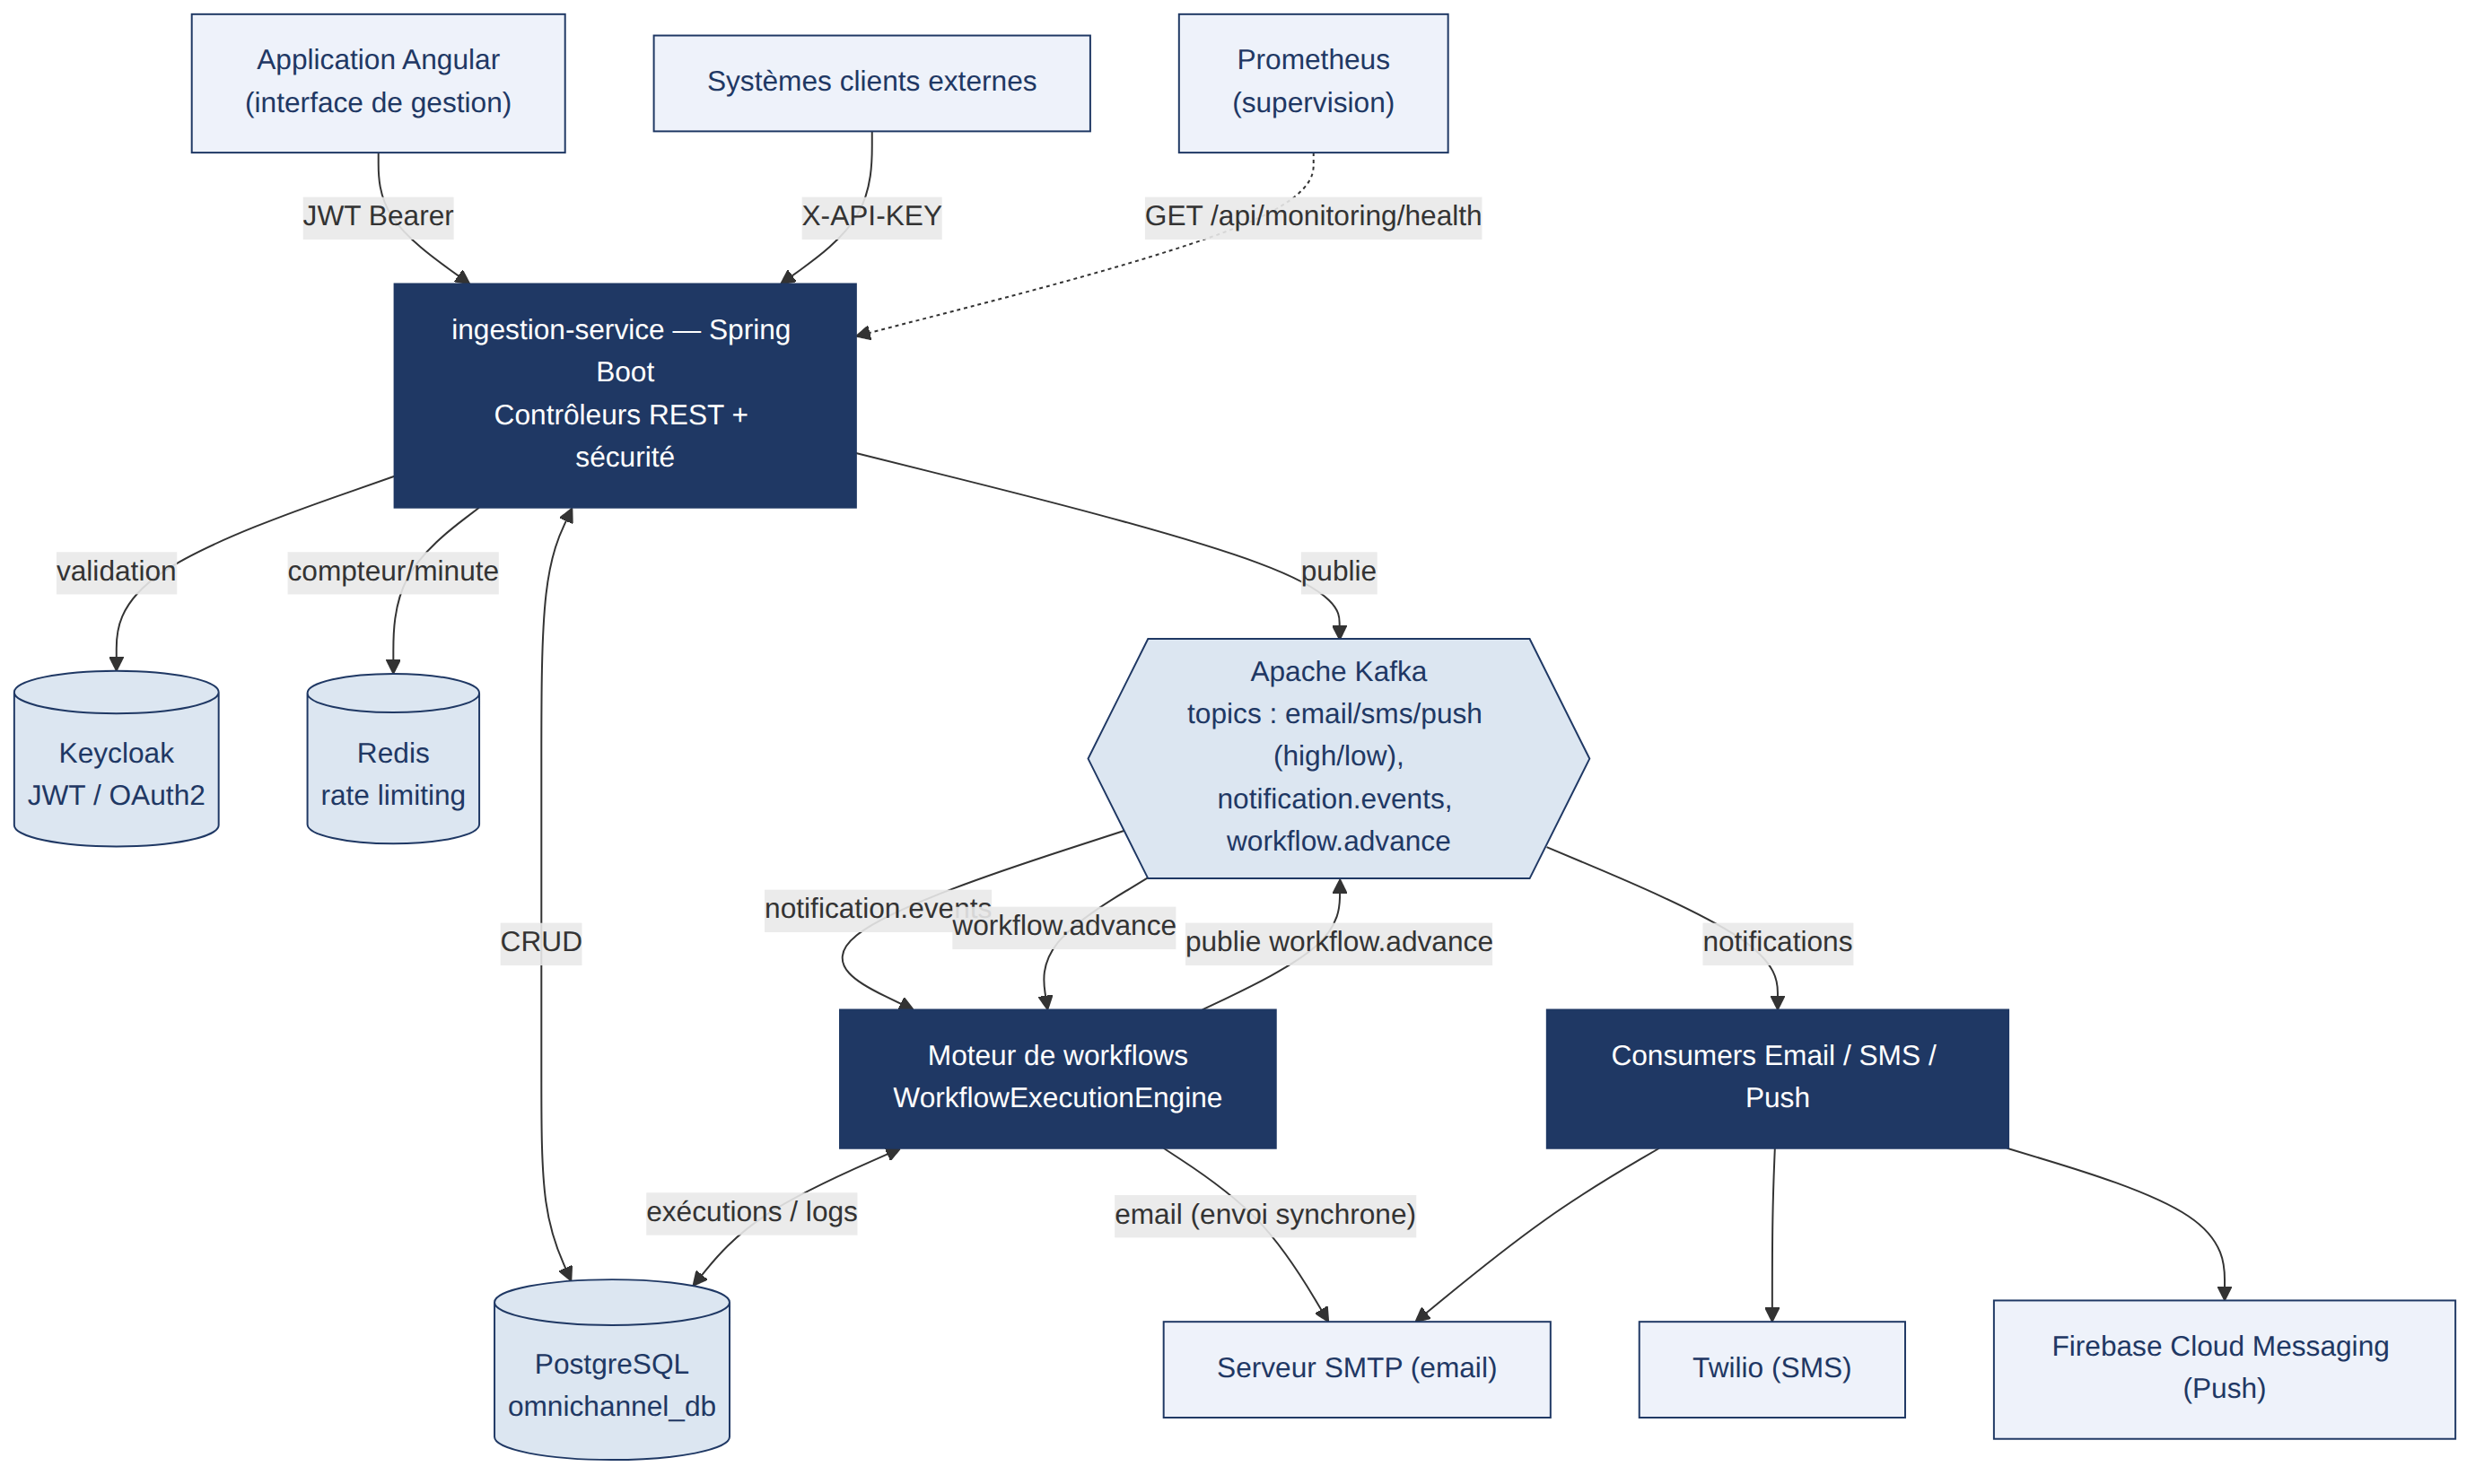
\includegraphics[width=0.9\textwidth]{figures/01-architecture.png}
  \caption{Architecture globale de la plateforme}
\end{figure}

Cette architecture découplée présente un double avantage : elle absorbe les pics de charge sans bloquer les appelants (le producteur n'attend jamais la fin du traitement), et elle isole les responsabilités --- ingestion, orchestration des workflows, acheminement par canal --- dans des composants indépendants, conformément aux exigences de performance et de scalabilité formulées au chapitre 2.

\section{Diagramme de cas d'utilisation}

Le diagramme suivant représente, sous forme de cas d'utilisation UML, les interactions identifiées au chapitre 2 entre les cinq acteurs de la plateforme et ses principales fonctionnalités. La relation « include » entre « Créer / modifier un workflow » et « Activer / dupliquer un workflow » illustre la validation structurelle du graphe (unicité du déclencheur, accessibilité de tous les n\oe uds, cohérence des conditions) systématiquement exécutée avant toute activation.

\begin{figure}[H]
  \centering
  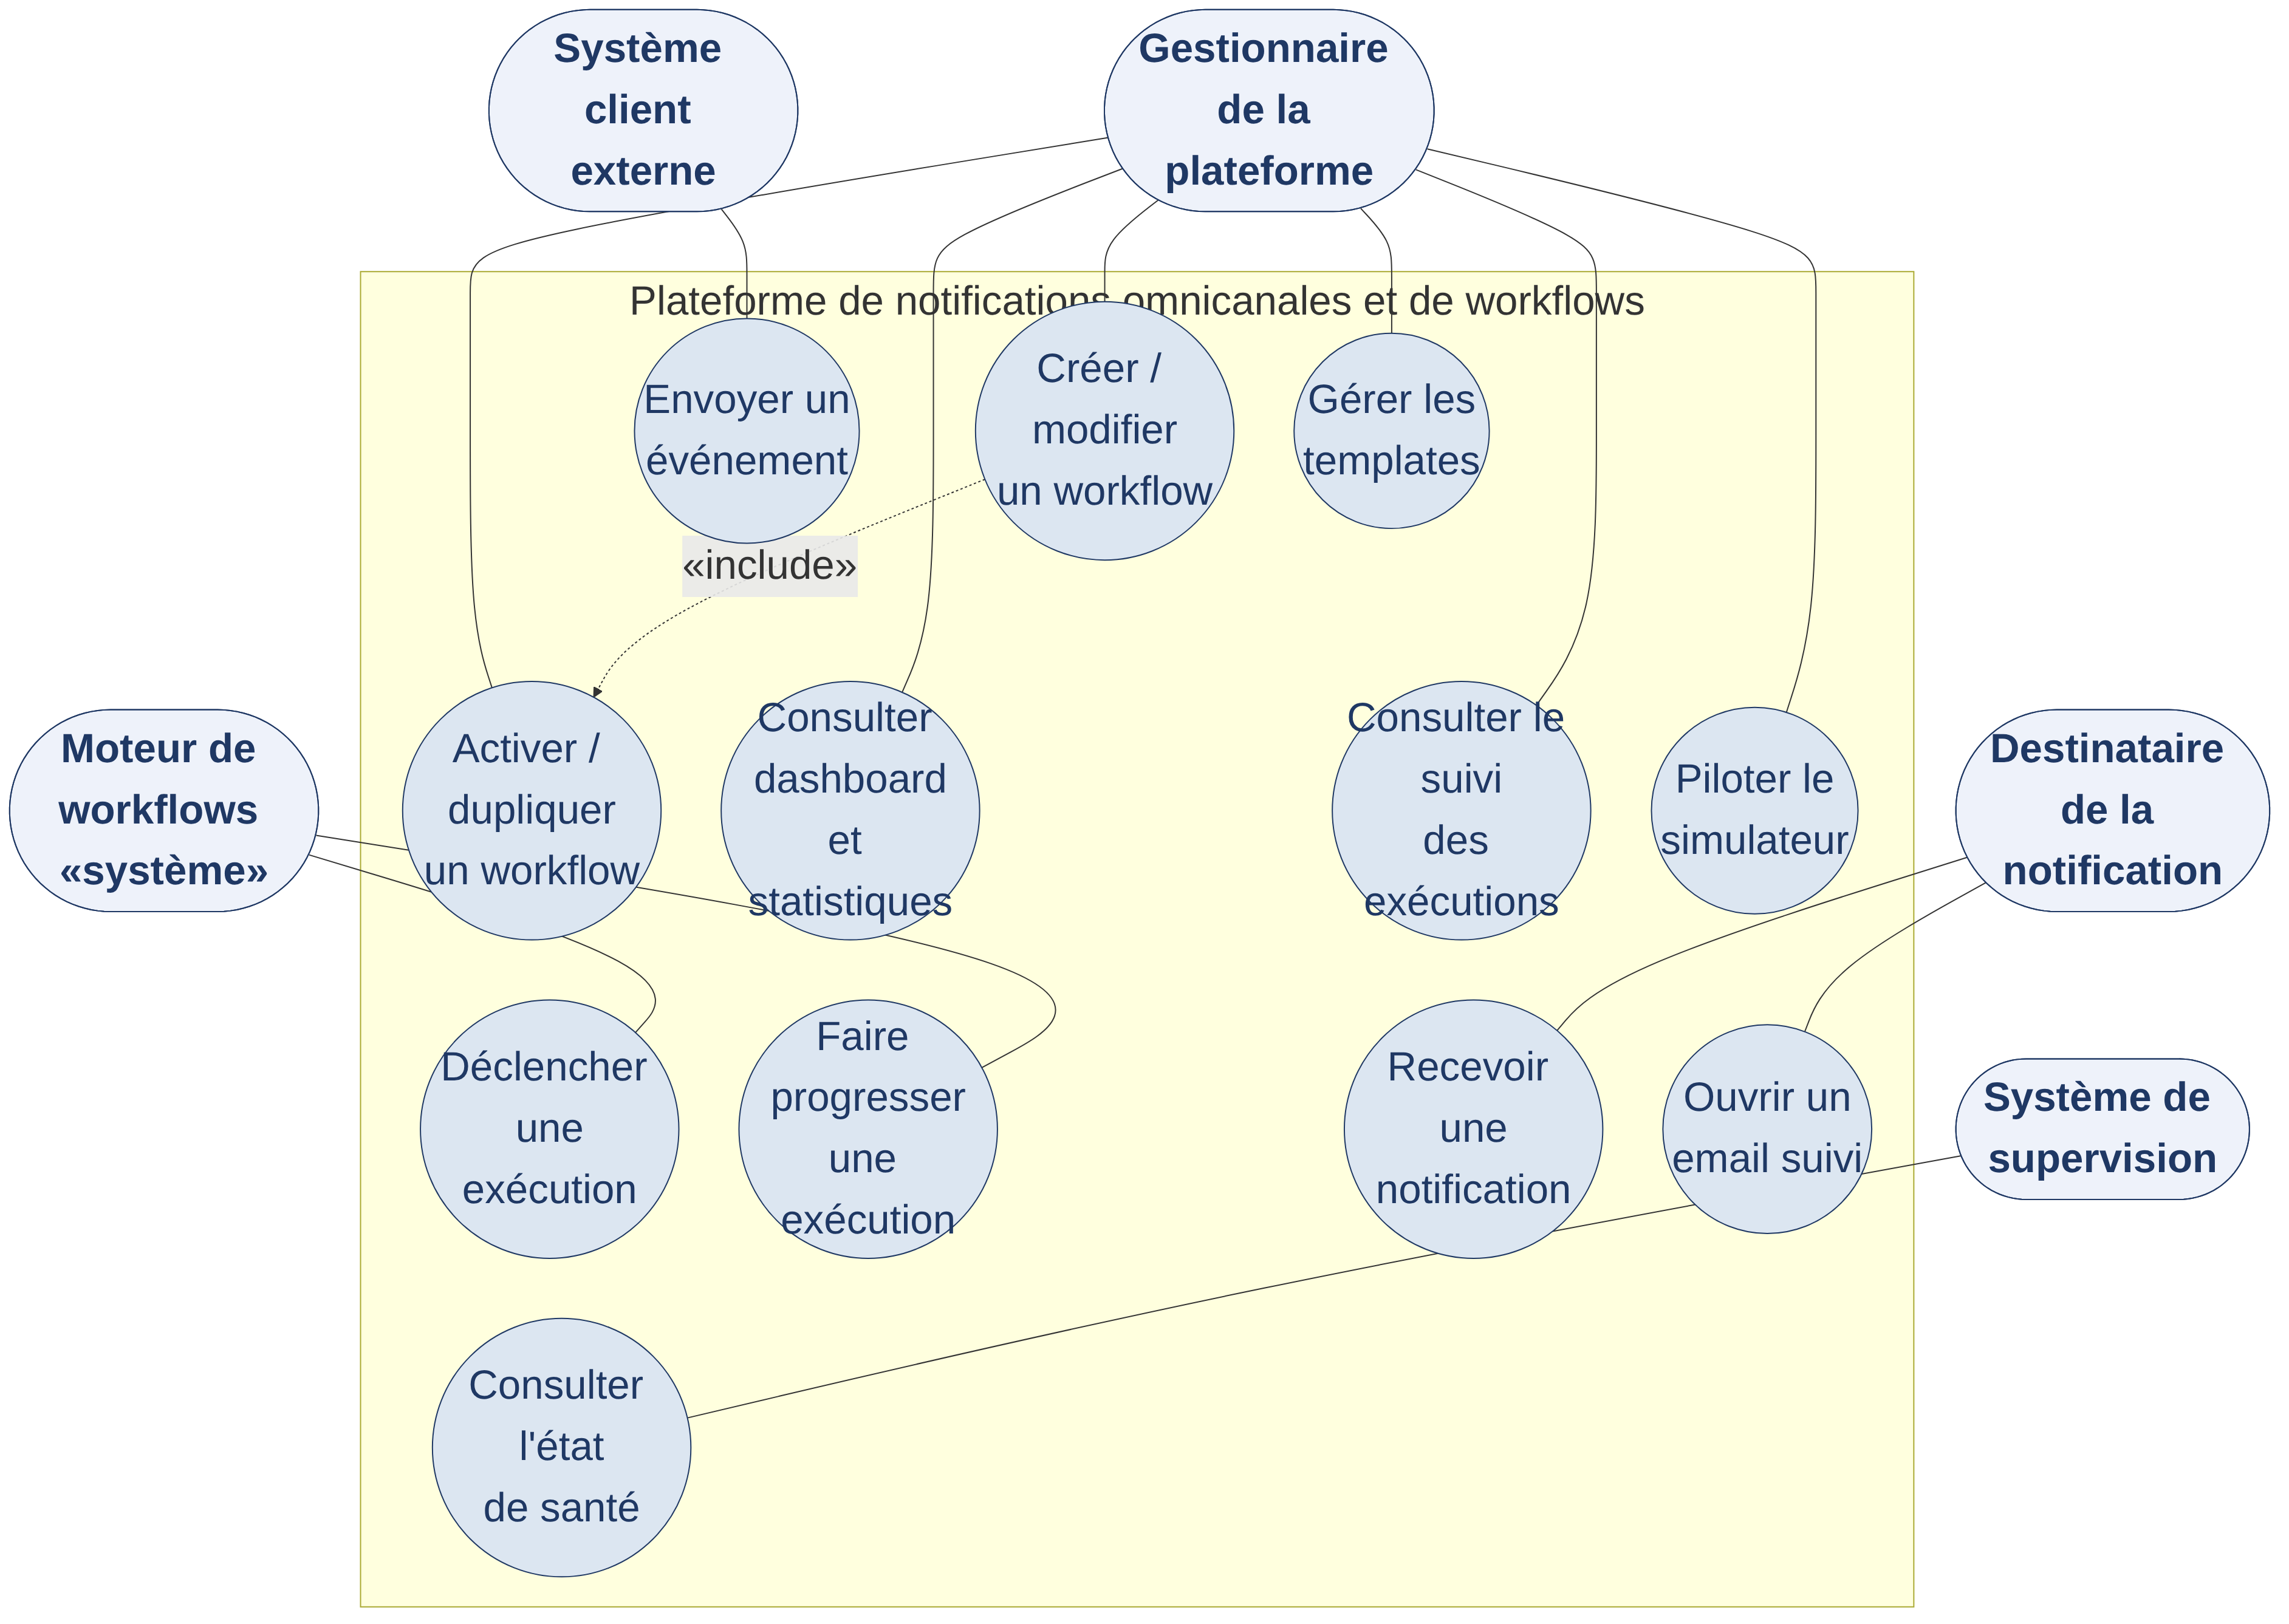
\includegraphics[width=0.92\textwidth]{figures/02-cas-utilisation.png}
  \caption{Diagramme de cas d'utilisation}
\end{figure}

\section{Diagrammes de séquence}

Deux scénarios ont été retenus pour illustrer le comportement dynamique du système : l'envoi direct d'une notification par un système client externe, et le déclenchement puis l'exécution complète d'un workflow événementiel.

\subsection{Envoi direct d'une notification}

Ce premier scénario illustre le chemin le plus simple de la plateforme : un système client externe authentifié par clé d'API soumet une notification, qui est validée, limitée en débit puis publiée sur Kafka de façon asynchrone, avant d'être effectivement acheminée par le consommateur du canal concerné, sous réserve des préférences de l'utilisateur et des éventuelles heures de silence.

\begin{figure}[H]
  \centering
  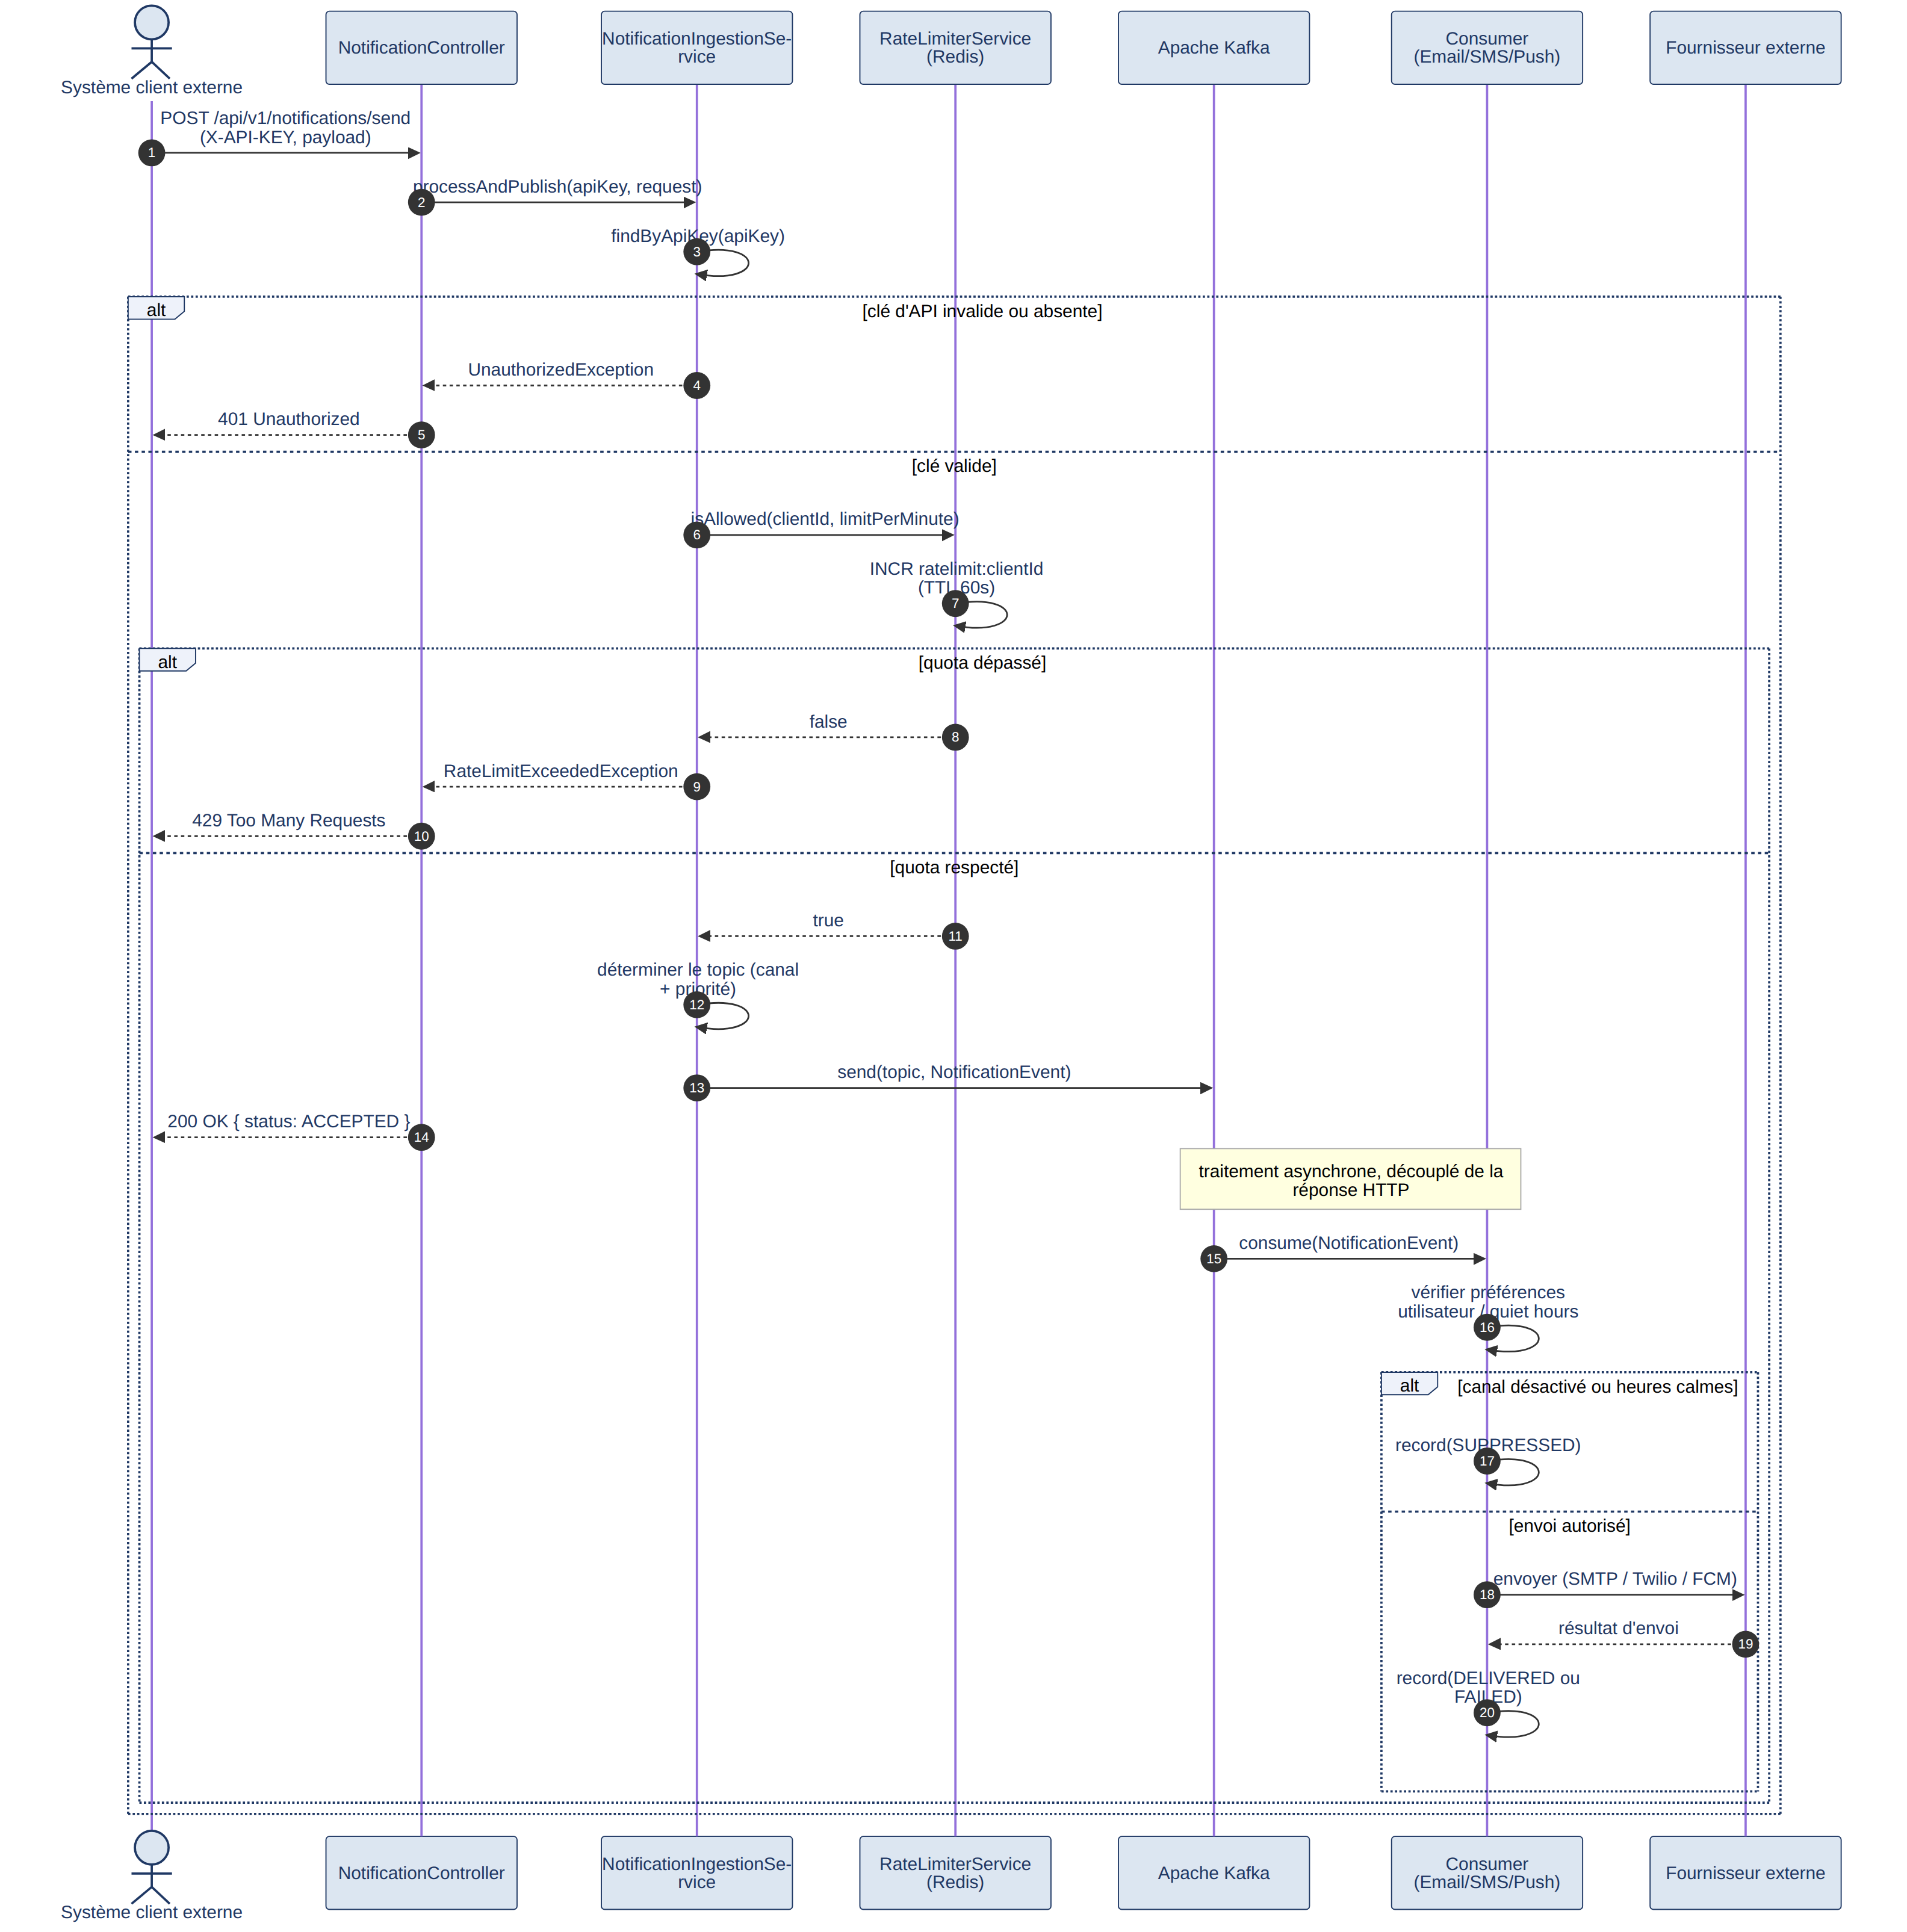
\includegraphics[width=0.72\textwidth]{figures/03-sequence-notification.png}
  \caption{Séquence --- Envoi et diffusion directe d'une notification}
\end{figure}

\subsection{Déclenchement et exécution d'un workflow}

Ce second scénario illustre le fonctionnement du moteur de workflows, de la publication d'un événement métier jusqu'à la terminaison de l'exécution qu'il déclenche. Il met en évidence le caractère strictement automatique de la création d'une exécution --- jamais lancée manuellement par un utilisateur --- ainsi que les trois comportements possibles d'un n\oe ud : poursuite immédiate (notification, condition), suspension programmée (n\oe ud d'attente, reprise ultérieure par le planificateur), ou terminaison (n\oe ud de fin).

\begin{figure}[H]
  \centering
  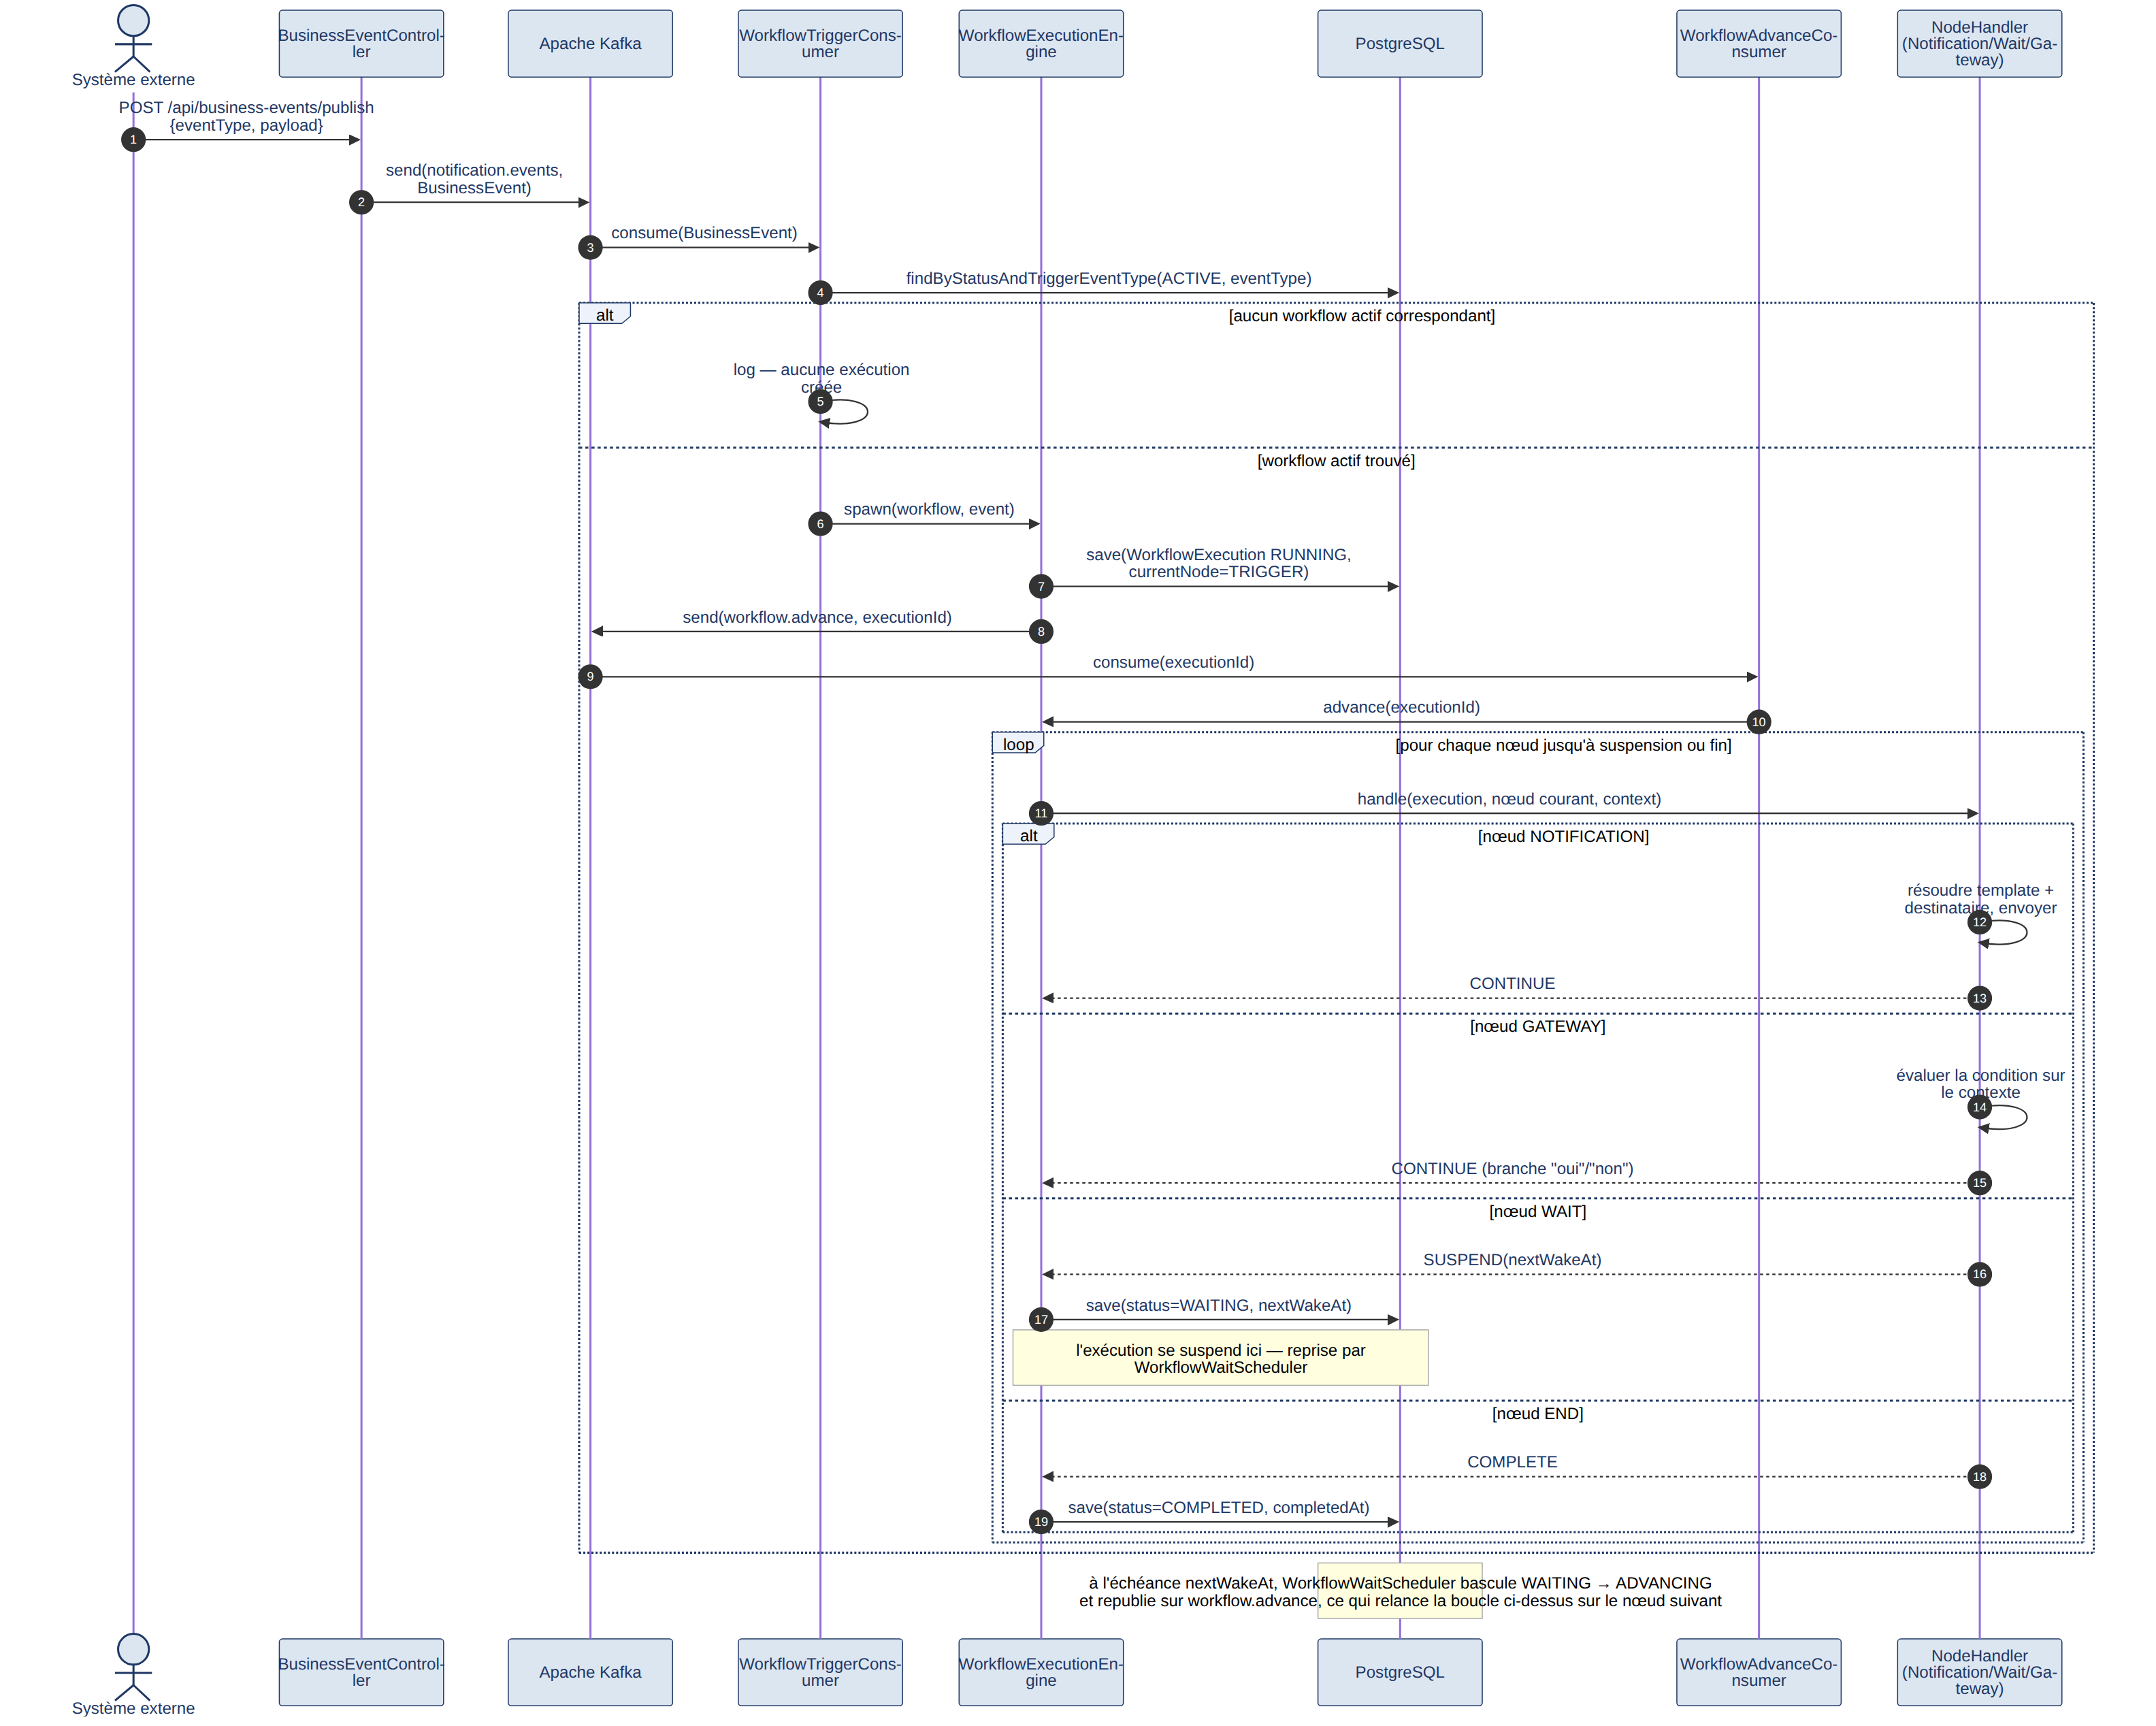
\includegraphics[width=0.8\textwidth]{figures/04-sequence-workflow.png}
  \caption{Séquence --- Déclenchement et exécution d'un workflow}
\end{figure}

\section{Diagramme de classes}

Le diagramme ci-dessous présente le modèle de domaine du backend. Il distingue les entités persistées (Workflow, WorkflowExecution, WorkflowExecutionLog, NotificationTemplate, ClientApp, UserPreference, NotificationLog) des éléments du graphe d'un workflow (NodeDef, EdgeDef), qui ne sont jamais persistés indépendamment : ils sont désérialisés à la volée depuis le champ JSON definitionJson de l'entité Workflow à chaque étape d'exécution.

\begin{figure}[H]
  \centering
  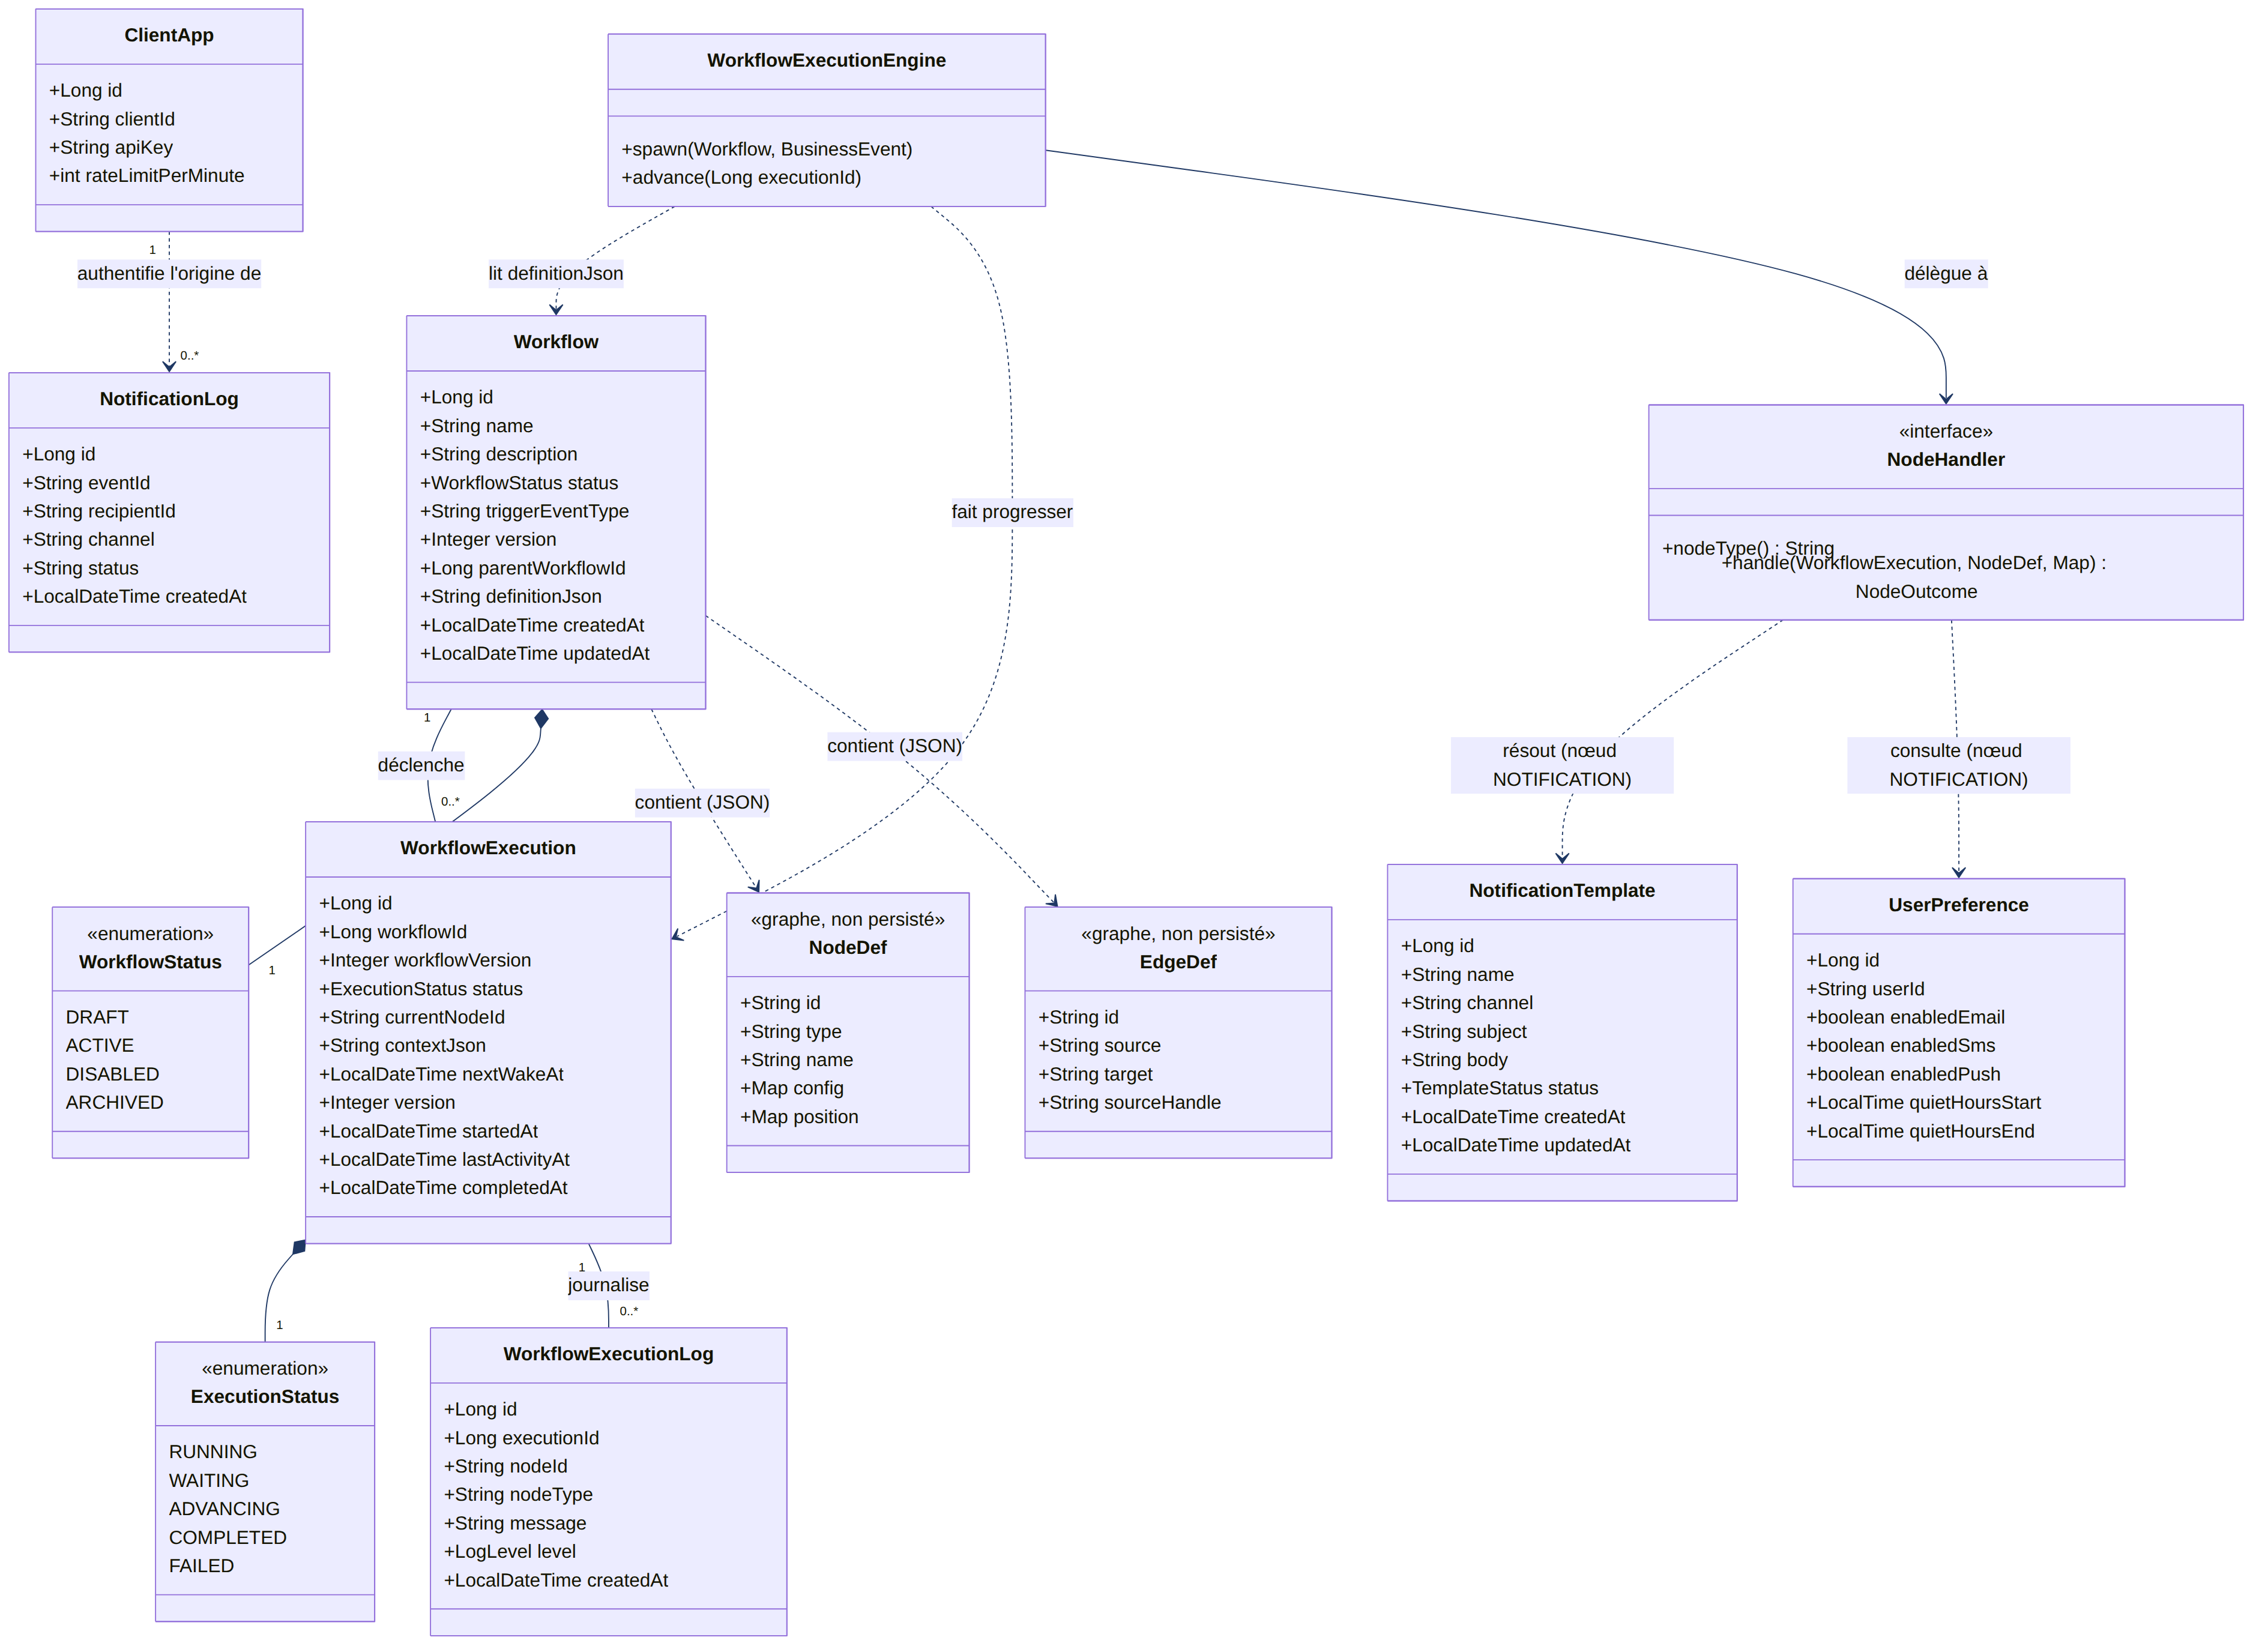
\includegraphics[width=0.92\textwidth]{figures/05-classes.png}
  \caption{Diagramme de classes du modèle de domaine}
\end{figure}

Deux choix de conception méritent d'être soulignés. D'une part, le versionnement des workflows suit une logique de copie sur écriture (copy-on-write) : modifier un workflow actif ne modifie jamais la ligne existante, mais crée une nouvelle version à l'état brouillon, référencée par parentWorkflowId --- garantissant qu'une exécution en cours reste toujours associée à la définition exacte sur laquelle elle a démarré (workflowVersion). D'autre part, chaque WorkflowExecution porte un champ de verrouillage optimiste (version), qui protège contre une double reprise de la même exécution lorsque plusieurs instances du moteur tournent en parallèle.

\section{Diagramme de composants}

Le diagramme suivant présente l'organisation en couches retenue, aussi bien côté frontend que backend. Côté frontend, les pages Angular s'appuient sur des services HTTP dédiés par domaine fonctionnel, eux-mêmes traversés par un intercepteur qui joint systématiquement le jeton JWT délivré par Keycloak à chaque requête. Côté backend, les contrôleurs REST délèguent aux services applicatifs et au moteur de workflows, qui s'appuient tous deux sur les repositories JPA pour la persistance et sur les producteurs/consommateurs Kafka pour l'intégration événementielle.

\begin{figure}[H]
  \centering
  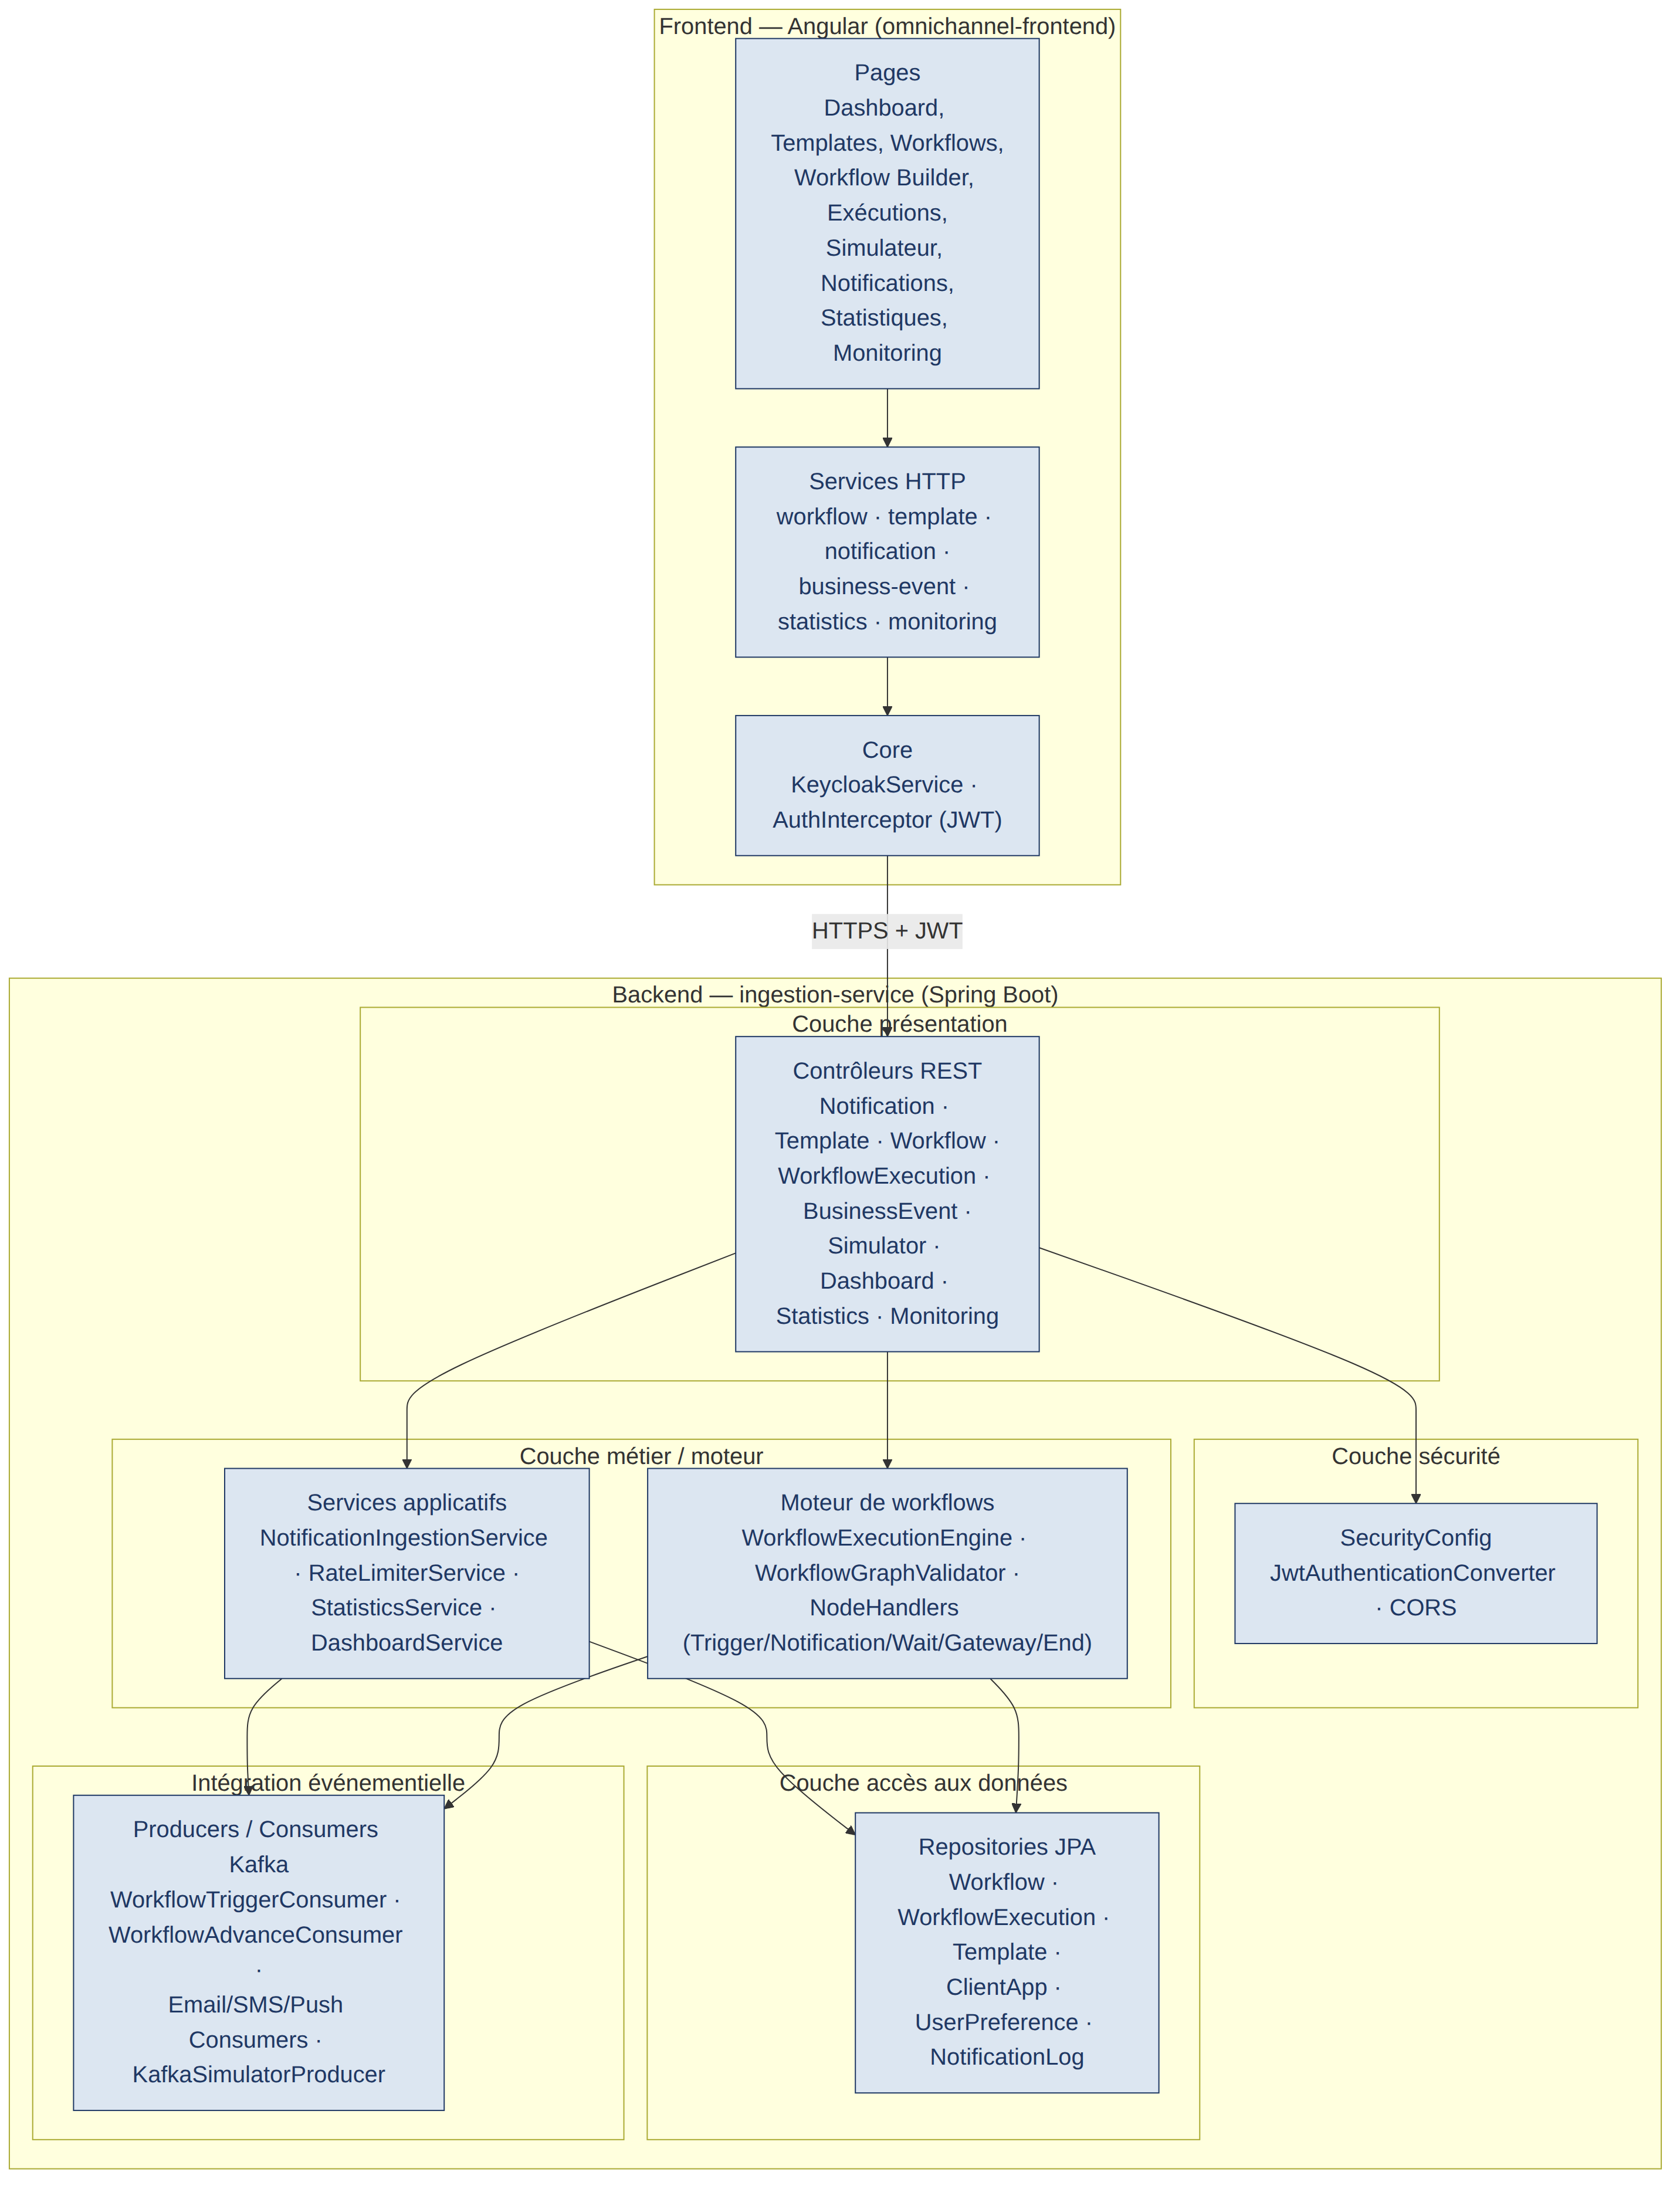
\includegraphics[width=0.62\textwidth]{figures/06-composants.png}
  \caption{Diagramme de composants}
\end{figure}

\section*{Conclusion}
\addcontentsline{toc}{section}{Conclusion}

Ce chapitre a présenté la conception technique de la plateforme : son architecture globale orientée événements, sa modélisation UML (cas d'utilisation, séquences, classes) ainsi que son organisation en composants. Cette conception constitue le plan directeur sur lequel s'appuie la réalisation effective de la solution, dont l'environnement et les outils de développement sont détaillés au chapitre suivant.

% ============================================================================
% Chapitre 4
% ============================================================================
\chapter{Environnement et outils de développement}

\section*{Introduction}
\addcontentsline{toc}{section}{Introduction}

Après avoir détaillé la conception de la plateforme au chapitre précédent, ce quatrième chapitre présente l'environnement et l'ensemble des outils mobilisés pour sa réalisation effective. Il couvre successivement l'environnement matériel et logiciel de développement, les technologies et frameworks retenus côté backend puis côté frontend, l'infrastructure et les middlewares sur lesquels repose la plateforme, les outils de conteneurisation et de supervision, ainsi que les outils de qualité et de test qui ont accompagné le développement de bout en bout. Chaque technologie présentée ici est directement issue du code source du projet (fichiers pom.xml, package.json, docker-compose.yml et configuration d'environnement) et non d'un choix générique : elle reflète fidèlement la stack effectivement mise en \oe uvre.

\section{Environnement matériel et logiciel}

Le développement de la plateforme n'a nécessité aucune ressource matérielle spécifique : une station de travail de développement standard, capable de faire tourner simultanément un IDE, une JVM et l'ensemble des conteneurs Docker de l'infrastructure (section 4.4), suffit.

\placeholder{Caractéristiques exactes de la ou des machines utilisées (processeur, RAM, système d'exploitation) à préciser si vous souhaitez les faire figurer ici --- elles n'ont pas d'incidence particulière sur la reproductibilité du projet, l'ensemble des services étant conteneurisé.}

Sur le plan logiciel, en revanche, plusieurs choix sont directement attestés par la configuration du projet : le backend a été développé sous IntelliJ IDEA --- le projet contient une configuration d'exécution Spring Boot dédiée (IngestionServiceApplication) ainsi qu'une intégration Git/GitHub avancée (recherche de pull requests) --- tandis que Visual Studio Code a également été utilisé, les deux sous-projets (ingestion-service et omnichannel-frontend) embarquant chacun une configuration .vscode (tâches de lancement, débogage, extension Angular Language Service recommandée). La gestion des dépendances et des builds repose sur Maven côté backend (via le wrapper mvnw, garantissant une version de Maven reproductible sans installation locale) et sur npm associé à l'Angular CLI côté frontend. Le versionnement du code source est assuré par Git, hébergé sur GitHub, avec un flux de travail basé sur les pull requests.

\begin{longtable}{@{}>{\raggedright\arraybackslash}p{0.28\textwidth}p{0.58\textwidth}@{}}
\caption{Environnement de développement}\\
\hline
\rowcolor{darkblue}\textcolor{white}{\textbf{Outil}} & \textcolor{white}{\textbf{Usage dans le projet}} \\
\hline
\endfirsthead
\hline
\rowcolor{darkblue}\textcolor{white}{\textbf{Outil}} & \textcolor{white}{\textbf{Usage dans le projet}} \\
\hline
\endhead
\hline
\endfoot
\textbf{IntelliJ IDEA} & IDE principal du développement backend (Java / Spring Boot), configuration d'exécution et de débogage dédiée \\
\hline
\textbf{Visual Studio Code} & Édition et débogage du frontend Angular (et, ponctuellement, du backend), avec l'extension Angular Language Service \\
\hline
\textbf{Maven (+ wrapper mvnw)} & Gestion des dépendances, compilation, exécution des tests et du calcul de couverture du backend \\
\hline
\textbf{npm + Angular CLI 19} & Gestion des dépendances, serveur de développement, build et exécution des tests du frontend \\
\hline
\textbf{Git / GitHub} & Gestion de versions et revue de code par pull requests \\
\hline
\textbf{Docker / Docker Compose} & Exécution reproductible de l'ensemble de l'infrastructure (sections 4.4 et 4.5) \\
\hline
\end{longtable}

\section{Technologies et frameworks backend}

Le backend \textit{ingestion-service} est développé en \textbf{Java 17}, au-dessus du framework \textbf{Spring Boot 3.3.3}, qui fournit l'ossature de l'application ainsi que l'ensemble des modules Spring nécessaires à ses différentes responsabilités.

\begin{itemize}
  \item \textbf{Spring Web} expose l'ensemble des contrôleurs REST de la plateforme (notifications, templates, workflows, exécutions, événements métier, simulateur, tableau de bord, statistiques, supervision).
  \item \textbf{Spring Data JPA} assure la persistance des entités du domaine (Workflow, WorkflowExecution, NotificationTemplate, ClientApp, UserPreference, NotificationLog…) vers PostgreSQL, avec un mappage JSON natif (jsonb) pour les champs definitionJson et contextJson.
  \item \textbf{Spring Security couplé à Spring OAuth2 Resource Server} sécurise les points de terminaison internes par validation de jetons JWT émis par Keycloak, avec un convertisseur d'autorités dédié qui traduit les rôles de royaume Keycloak (realm\_access.roles) en rôles Spring Security.
  \item \textbf{Spring Kafka} fournit à la fois les producteurs (publication des événements et notifications) et les consommateurs (\texttt{@KafkaListener}) qui implémentent le moteur de workflows et l'acheminement omnicanal.
  \item \textbf{Spring Data Redis} est utilisé par le service de limitation de débit (rate limiting par client, avec expiration automatique des compteurs).
  \item \textbf{Spring Boot Mail} gère l'envoi des notifications par courrier électronique, y compris l'insertion du pixel de suivi d'ouverture.
  \item \textbf{Spring Boot Actuator et Micrometer (registre Prometheus)} exposent l'état de santé et les métriques applicatives, consommées par Prometheus (section 4.5).
  \item \textbf{Lombok 1.18.36} réduit le code répétitif (accesseurs, constructeurs, builders) des entités et DTO.
\end{itemize}

\begin{longtable}{@{}>{\raggedright\arraybackslash}p{0.34\textwidth}p{0.52\textwidth}@{}}
\caption{Technologies et frameworks --- Backend}\\
\hline
\rowcolor{darkblue}\textcolor{white}{\textbf{Technologie}} & \textcolor{white}{\textbf{Rôle dans le projet}} \\
\hline
\endfirsthead
\hline
\rowcolor{darkblue}\textcolor{white}{\textbf{Technologie}} & \textcolor{white}{\textbf{Rôle dans le projet}} \\
\hline
\endhead
\hline
\endfoot
Java 17 & Langage du backend \\
\hline
Spring Boot 3.3.3 & Framework applicatif principal \\
\hline
Spring Web & Contrôleurs REST \\
\hline
Spring Data JPA + PostgreSQL & Persistance du modèle de domaine \\
\hline
Spring Security + OAuth2 Resource Server & Authentification JWT (Keycloak) \\
\hline
Spring Kafka & Producteurs / consommateurs d'événements \\
\hline
Spring Data Redis & Limitation de débit (rate limiting) \\
\hline
Spring Boot Mail & Envoi des notifications par email \\
\hline
Spring Boot Actuator + Micrometer & Santé applicative et métriques Prometheus \\
\hline
Lombok & Réduction du code répétitif \\
\hline
\end{longtable}

\section{Technologies frontend}

Le frontend \textit{omnichannel-frontend} est développé avec \textbf{Angular 19} et \textbf{TypeScript 5.6}, en s'appuyant exclusivement sur des \textbf{composants autonomes (standalone components)} : l'application ne comporte aucun NgModule, le bootstrap (ApplicationConfig) et le routage (chaque page étant chargée à la demande via loadComponent) suivant intégralement l'approche standalone introduite par les versions récentes d'Angular.

\begin{itemize}
  \item \textbf{Tailwind CSS 4} (intégré via @tailwindcss/postcss) fournit l'ensemble de la mise en forme utilitaire de l'interface, complété par SCSS pour les styles propres à certains composants.
  \item \textbf{keycloak-js 24} implémente, côté client, le flux d'authentification OpenID Connect auprès du même serveur Keycloak que le backend ; un intercepteur HTTP (AuthInterceptor) joint automatiquement le jeton obtenu à chaque appel API, et un provideAppInitializer bloque le démarrage de l'application jusqu'à authentification complète.
  \item \textbf{ngx-vflow} est la bibliothèque de graphe interactif utilisée par l'éditeur visuel de workflows (workflow builder) pour le glisser-déposer des n\oe uds et le tracé des transitions entre eux.
  \item \textbf{lucide-angular} fournit le jeu d'icônes utilisé à travers l'ensemble de l'interface.
  \item \textbf{RxJS 7.8} structure la gestion asynchrone des appels HTTP et des flux de données au sein des services Angular.
\end{itemize}

\begin{longtable}{@{}>{\raggedright\arraybackslash}p{0.34\textwidth}p{0.52\textwidth}@{}}
\caption{Technologies et frameworks --- Frontend}\\
\hline
\rowcolor{darkblue}\textcolor{white}{\textbf{Technologie}} & \textcolor{white}{\textbf{Rôle dans le projet}} \\
\hline
\endfirsthead
\hline
\rowcolor{darkblue}\textcolor{white}{\textbf{Technologie}} & \textcolor{white}{\textbf{Rôle dans le projet}} \\
\hline
\endhead
\hline
\endfoot
Angular 19 (standalone) & Framework frontend, sans NgModule \\
\hline
TypeScript 5.6 & Langage du frontend \\
\hline
Tailwind CSS 4 + SCSS & Mise en forme de l'interface \\
\hline
keycloak-js 24 & Authentification OpenID Connect côté client \\
\hline
ngx-vflow & Éditeur visuel de workflows (n\oe uds / transitions) \\
\hline
lucide-angular & Jeu d'icônes de l'interface \\
\hline
RxJS 7.8 & Programmation réactive / appels HTTP \\
\hline
Angular CLI 19 & Outillage de build, de serveur de dev et de test \\
\hline
\end{longtable}

\section{Infrastructure et middleware}

L'ensemble de l'infrastructure nécessaire à l'exécution de la plateforme en environnement de développement est décrit dans un unique fichier docker-compose.yml, garantissant sa reproductibilité intégrale sur n'importe quelle machine disposant de Docker.

\begin{itemize}
  \item \textbf{Apache Kafka} (accompagné de Zookeeper) constitue le bus d'événements central de la plateforme, support de l'ensemble des topics de notifications et du moteur de workflows (chapitre 3).
  \item \textbf{PostgreSQL} est le système de gestion de base de données relationnelle unique de la plateforme (base omnichannel\_db), retenu notamment pour son support natif du type jsonb utilisé par le moteur de workflows.
  \item \textbf{Redis} sert de magasin de compteurs pour la limitation de débit par client (rate limiting), avec expiration automatique.
  \item \textbf{Mailpit} simule un serveur SMTP en environnement de développement et capture les emails envoyés (notamment ceux du moteur de workflows) dans une interface web dédiée, sans jamais les délivrer à un véritable destinataire.
  \item \textbf{Keycloak} assure la gestion des identités et des accès (IAM) de la plateforme au moyen du protocole OpenID Connect / OAuth2, avec un royaume (realm) dédié importé automatiquement au démarrage et définissant les rôles ADMIN et SERVICE\_CLIENT.
\end{itemize}

\begin{longtable}{@{}>{\raggedright\arraybackslash}p{0.24\textwidth}p{0.62\textwidth}@{}}
\caption{Services d'infrastructure orchestrés par Docker Compose}\\
\hline
\rowcolor{darkblue}\textcolor{white}{\textbf{Service}} & \textcolor{white}{\textbf{Image Docker -- rôle -- port exposé}} \\
\hline
\endfirsthead
\hline
\rowcolor{darkblue}\textcolor{white}{\textbf{Service}} & \textcolor{white}{\textbf{Image Docker -- rôle -- port exposé}} \\
\hline
\endhead
\hline
\endfoot
\textbf{PostgreSQL} & postgres:15-alpine --- base de données omnichannel\_db --- port 5433 \\
\hline
\textbf{Redis} & redis:7-alpine --- limitation de débit --- port 6379 \\
\hline
\textbf{Mailpit} & axllent/mailpit --- serveur SMTP de test + interface web --- ports 1025 / 8025 \\
\hline
\textbf{Zookeeper} & confluentinc/cp-zookeeper:7.5.0 --- coordination du cluster Kafka \\
\hline
\textbf{Apache Kafka} & confluentinc/cp-kafka:7.5.0 --- bus d'événements --- port 9092 \\
\hline
\textbf{Kafka UI} & provectuslabs/kafka-ui --- supervision des topics Kafka --- port 8085 \\
\hline
\textbf{Keycloak} & quay.io/keycloak/keycloak:24.0.2 --- gestion des identités (JWT/OIDC) --- port 8081 \\
\hline
\textbf{Prometheus} & prom/prometheus --- collecte des métriques applicatives --- port 9090 \\
\hline
\end{longtable}

\section{Outils de conteneurisation et de supervision}

\textbf{Docker et Docker Compose} constituent la pierre angulaire de la reproductibilité de l'environnement : l'ensemble des huit services listés au tableau 4.4 est décrit dans un unique fichier docker-compose.yml et démarré par une seule commande, sans installation manuelle de PostgreSQL, Kafka ou Keycloak sur la machine hôte. Chaque service dispose de son propre conteneur, isolé, versionné par une étiquette d'image précise, ce qui élimine les écarts d'environnement entre les postes de développement.

\textbf{Kafka UI} offre un tableau de bord web (port 8085) permettant d'inspecter en temps réel les topics Kafka, leurs partitions et les messages qui y transitent --- un outil précieux pour déboguer visuellement le flux d'événements sans écrire de code de consommation ad hoc.

\textbf{Prometheus} collecte, toutes les 5 secondes, les métriques exposées par ingestion-service sur son point de terminaison /actuator/prometheus (activé via Spring Boot Actuator et Micrometer), couvrant à la fois des métriques techniques (JVM, requêtes HTTP) et l'état de santé applicatif. Il constitue le pendant automatisé du point de terminaison public de supervision présenté au chapitre 2.

\section{Outils de qualité et de test}

La qualité du code a été mesurée et contrôlée en continu tout au long du développement, à l'aide d'outils distincts mais complémentaires côté backend et frontend.

\begin{itemize}
  \item \textbf{SonarQube} analyse les deux sous-projets séparément, sous deux clés de projet distinctes (omnichannel-backend et omnichannel-frontend) : le backend est scanné via le plugin Maven Sonar, à partir du rapport XML généré par JaCoCo ; le frontend est scanné via la CLI sonar-scanner, à partir d'un rapport de couverture au format LCOV généré par Karma. C'est cette double analyse qui a permis d'établir les taux de couverture de 87,4~\% (backend) et 93,0~\% (frontend) présentés au chapitre 5.
  \item \textbf{JaCoCo} instrumente l'exécution des tests backend (agent attaché avant Surefire) pour produire le rapport de couverture consommé par SonarQube.
  \item \textbf{JUnit 5 et Mockito} constituent la base des tests unitaires et d'intégration du backend (via spring-boot-starter-test et spring-kafka-test pour les tests impliquant Kafka), détaillés au chapitre 5.
  \item \textbf{Jasmine et Karma} exécutent les tests unitaires du frontend Angular, avec karma-coverage pour la mesure de couverture et un lancement en mode navigateur headless (Chrome sans interface graphique), adapté à une exécution automatisée.
  \item \textbf{GitHub Actions} automatise l'exécution de l'ensemble de ces tests à chaque push et à chaque pull request sur la branche principale, via un pipeline d'intégration continue à deux jobs distincts : l'un installe un JDK 17 (Temurin) et exécute mvn clean test pour le backend, l'autre installe Node.js 20 et exécute les tests Angular en Chrome headless pour le frontend --- garantissant qu'aucune régression n'est fusionnée sans que la suite de tests ne passe intégralement.
\end{itemize}

\begin{longtable}{@{}>{\raggedright\arraybackslash}p{0.34\textwidth}p{0.52\textwidth}@{}}
\caption{Outils de qualité et de test}\\
\hline
\rowcolor{darkblue}\textcolor{white}{\textbf{Outil}} & \textcolor{white}{\textbf{Rôle dans le projet}} \\
\hline
\endfirsthead
\hline
\rowcolor{darkblue}\textcolor{white}{\textbf{Outil}} & \textcolor{white}{\textbf{Rôle dans le projet}} \\
\hline
\endhead
\hline
\endfoot
SonarQube & Analyse statique et suivi de la couverture de code (2 projets distincts) \\
\hline
JaCoCo & Génération du rapport de couverture backend (XML) \\
\hline
JUnit 5 + Mockito & Tests unitaires et d'intégration backend \\
\hline
Jasmine + Karma & Tests unitaires frontend, couverture LCOV \\
\hline
GitHub Actions & Intégration continue (tests backend + frontend à chaque push/PR) \\
\hline
\end{longtable}

\section*{Conclusion}
\addcontentsline{toc}{section}{Conclusion}

Ce chapitre a présenté l'ensemble de l'environnement et des outils mobilisés pour la réalisation de la plateforme : IDE et outils de build, frameworks backend et frontend, infrastructure conteneurisée et outils de supervision, ainsi que la chaîne complète d'assurance qualité, de l'analyse statique à l'intégration continue. Cette stack technique cohérente et entièrement reproductible a constitué le socle sur lequel s'appuie la réalisation présentée au chapitre suivant, qui détaille les fonctionnalités développées, la stratégie de test mise en \oe uvre et les résultats de couverture de code obtenus.

% ============================================================================
% Chapitre 5
% ============================================================================
\chapter{Réalisation, tests et couverture de code}

\section*{Introduction}
\addcontentsline{toc}{section}{Introduction}

Ce cinquième et dernier chapitre présente la phase de réalisation et de validation de la plateforme. Il décrit d'abord les principales interfaces graphiques développées côté frontend, qui matérialisent les besoins fonctionnels spécifiés au chapitre 2. Il détaille ensuite la stratégie de test mise en \oe uvre, aussi bien côté backend que côté frontend, ainsi que la démarche suivie pour valider manuellement le comportement de l'API. Il présente enfin les résultats de qualité et de couverture de code obtenus via SonarQube, qui viennent objectiver la robustesse du travail réalisé.

\section{Principales interfaces graphiques}

Le frontend omnichannel-frontend (chapitre 4) expose, derrière une authentification Keycloak, une console d'administration organisée autour d'une barre de navigation latérale (Admin Console) donnant accès à huit espaces : Dashboard, Templates, Cinématiques (Workflows), Exécutions, Simulateur d'événements, Notifications, Statistiques et Monitoring. Les paragraphes suivants décrivent les quatre écrans les plus représentatifs de la valeur fonctionnelle de la plateforme.

\placeholder{Aucune capture d'écran réelle n'a été insérée dans cette version du rapport : l'environnement de rédaction ne permettait pas de lancer la stack complète (Docker, Keycloak, Postgres, Kafka) et le serveur de développement Angular pour produire des captures authentiques. Les descriptions ci-dessous sont en revanche fidèles au code source réel des composants (templates HTML) et il est vivement recommandé de les remplacer par de véritables captures d'écran avant l'impression finale du rapport.}

\subsection{Tableau de bord et statistiques}

La page Dashboard (« Dashboard \& Statistiques ») constitue l'écran d'accueil de la console. Son en-tête affiche un badge d'état « Système Opérationnel » ainsi que deux actions rapides, « Envoi Simulé » et « Rafraîchir ». Le corps de la page présente quatre cartes de métriques agrégées (volumes et taux clés de la plateforme) suivies d'un tableau des notifications récentes, dont chaque ligne affiche un badge de statut coloré selon une convention cohérente sur l'ensemble de l'application : vert émeraude pour les notifications livrées (Delivered), ambre pour celles en attente (Pending) et rouge rosé pour les échecs (Failed).

La page Statistiques (« Statistiques de Performance »), accessible séparément dans la navigation, approfondit cette vue d'ensemble à travers quatre indicateurs clés --- volume global, taux de livraison, taux d'ouverture et taux de clic --- puis un tableau détaillant la performance par canal (Email, SMS, Push). Deux précisions méthodologiques y sont affichées directement dans l'interface, par souci de transparence envers l'utilisateur : le taux d'ouverture n'est mesurable que pour les emails envoyés dans le cadre d'un workflow (pixel de suivi inséré par le moteur), et le taux de clic est explicitement annoncé comme non instrumenté (« Aucun suivi de clic implémenté ») --- un point de cohérence avec la limitation déjà signalée au chapitre 2 (section 2.5.7, Traçabilité).

\subsection{Éditeur visuel de workflows (Workflow Builder)}

L'écran Cinématiques (Workflows) permet de créer, modifier et activer les workflows décrits au chapitre 3. Son composant central est un éditeur de graphe interactif construit avec \textit{ngx-vflow} (section 4.3) : une palette latérale de n\oe uds, regroupés par catégorie, propose les cinq types de n\oe uds du moteur --- Trigger, Notification, Wait, Gateway et End --- que l'utilisateur glisse-dépose sur le canevas puis relie entre eux pour définir la logique conditionnelle du workflow. Chaque n\oe ud déposé peut être configuré individuellement (canal et template pour un n\oe ud Notification, durée pour un n\oe ud Wait, condition pour un n\oe ud Gateway), conformément au modèle NodeDef/EdgeDef présenté au diagramme de classes (figure 3.5).

Une fois le graphe ainsi construit validé, l'action « Enregistrer » persiste le workflow à l'état DRAFT ; l'action « Activer » le fait basculer à l'état ACTIVE, seul état dans lequel il peut effectivement être déclenché par un événement métier entrant (section 3.4). Un badge de statut coloré (DRAFT / ACTIVE / DISABLED / ARCHIVED) rappelle en permanence l'état courant du workflow affiché.

\subsection{Simulateur d'événements métier}

La page Simulateur d'événements métier permet de publier manuellement un événement métier vers la plateforme, sans dépendre d'un système externe réel --- un outil essentiel aussi bien pour la démonstration du projet que pour le test bout-en-bout des workflows. Son formulaire de gauche propose un choix entre des scénarios prédéfinis (presets) et un mode libre, dans lequel l'utilisateur saisit lui-même le type d'événement et un payload JSON personnalisé, avant de déclencher la publication via le bouton « Publier l'événement ». Le panneau de droite conserve un historique de session des événements publiés, chacun affichant un badge de statut retraçant si un workflow a effectivement été déclenché en réponse. Cet écran est distinct du simulateur bas niveau accessible depuis le Dashboard : il agit au niveau métier (événements), là où celui du Dashboard agit au niveau de l'envoi direct d'une notification unitaire (flux décrit à la figure 3.3).

\subsection{Suivi des exécutions de workflows}

La page de détail d'une exécution (accessible depuis la liste des Exécutions) identifie chaque instance par un identifiant du type « EXEC-\{id\} », accompagné d'un badge reflétant son état courant (RUNNING, WAITING, ADVANCING, COMPLETED ou FAILED --- cf. énumération ExecutionStatus, figure 3.5) et d'un fil d'Ariane de navigation. Quatre cartes de métadonnées résument l'exécution (workflow d'origine, version, dates de démarrage et de dernière activité). Le corps de la page adopte une disposition en deux colonnes : à gauche, une timeline chronologique de l'exécution, où chaque entrée du journal (WorkflowExecutionLog) est représentée par un point coloré selon son niveau (LogLevel) ; à droite, le contexte d'exécution complet (contextJson), affiché sous forme de JSON mis en forme, qui permet d'inspecter précisément les données ayant transité à chaque étape du workflow. Cet écran constitue l'outil de diagnostic principal pour comprendre a posteriori le déroulement --- normal ou en échec --- d'une instance de workflow, en cohérence avec l'exigence de traçabilité formulée au chapitre 2.

\section{Stratégie de test et de validation}

La fiabilité de la plateforme a été validée à plusieurs niveaux complémentaires : des tests automatisés unitaires et d'intégration côté backend, des tests automatisés unitaires côté frontend, ainsi qu'une validation manuelle du comportement de bout en bout de l'API et des workflows.

\subsection{Tests backend --- JUnit 5 et Mockito}

Le backend ingestion-service s'appuie sur JUnit 5 et Mockito (section 4.6) pour ses tests unitaires et d'intégration, complétés par spring-kafka-test pour les scénarios impliquant la production ou la consommation de messages Kafka. Au moment de la rédaction de ce rapport, la suite de tests backend compte \textbf{42 classes de test}, totalisant \textbf{255 méthodes annotées @Test}, couvrant notamment : la validation des règles métier des services applicatifs (NotificationIngestionService, RateLimiterService, StatisticsService, DashboardService), la logique du moteur de workflows (WorkflowExecutionEngine, WorkflowGraphValidator, les différents NodeHandler), les contrôleurs REST (via MockMvc), ainsi que les consommateurs et producteurs Kafka.

Ces tests s'exécutent automatiquement à chaque build Maven (mvn clean test) et sont instrumentés par JaCoCo pour produire le rapport de couverture consommé par SonarQube (section 5.3).

\subsection{Tests frontend --- Jasmine et Karma}

Le frontend omnichannel-frontend s'appuie sur Jasmine et Karma (section 4.6), exécutés en mode Chrome headless. Au moment de la rédaction de ce rapport, la suite de tests frontend compte \textbf{34 fichiers de spécification} (*.spec.ts), totalisant environ \textbf{268 appels it()}, couvrant les composants de pages (Dashboard, Statistiques, Simulateur d'événements, détail d'exécution, Workflow Builder…), les services HTTP (workflow, template, notification, business-event, statistics, monitoring) ainsi que les éléments transverses (intercepteur d'authentification, garde de route). La couverture obtenue est mesurée par karma-coverage et exportée au format LCOV pour analyse SonarQube.

\subsection{Validation manuelle de l'API et des workflows}

\placeholder{Point de vigilance : la consigne initiale de ce chapitre mentionnait une validation de l'API via Postman/Swagger. La vérification du code source (pom.xml du backend, absence de dépendance springdoc-openapi malgré des chemins /v3/api-docs et /swagger-ui réservés -- mais inutilisés -- dans SecurityConfig ; absence de toute collection Postman dans le dépôt) montre qu'aucune documentation Swagger/OpenAPI ni collection Postman n'a été mise en place sur ce projet. La validation manuelle de bout en bout a en réalité été effectuée par des appels HTTP directs (curl) et par l'utilisation de l'interface elle-même, comme décrit ci-dessous. Ce paragraphe restitue donc fidèlement la méthode réellement employée plutôt que la méthode initialement suggérée.}

En complément des tests automatisés, chaque fonctionnalité majeure a fait l'objet d'une validation manuelle de bout en bout, combinant appels HTTP directs (curl) sur les points de terminaison REST du backend et navigation dans les écrans de la console d'administration. Un scénario type de validation consiste, par exemple, à créer un template de notification, construire un workflow par glisser-déposer dans le Workflow Builder puis l'activer, publier un événement métier correspondant depuis le Simulateur d'événements, et observer la progression de l'exécution créée (RUNNING $\rightarrow$ WAITING $\rightarrow$ COMPLETED) dans l'écran de suivi des exécutions --- la transition WAITING $\rightarrow$ COMPLETED d'un n\oe ud Gateway étant elle-même déclenchée par l'ouverture réelle de l'email envoyé, via le pixel de suivi. Cette démarche a permis de valider empiriquement, sur des scénarios réels, l'ensemble de la chaîne événement $\rightarrow$ moteur de workflows $\rightarrow$ notification $\rightarrow$ suivi, au-delà de ce que couvrent isolément les tests unitaires.

\subsection{Intégration continue}

L'ensemble de ces tests automatisés (backend et frontend) est rejoué automatiquement par le pipeline GitHub Actions (section 4.6) à chaque push et à chaque pull request sur la branche principale, au travers de deux jobs parallèles et indépendants. Cette automatisation garantit qu'aucune régression fonctionnelle n'est fusionnée dans le code de référence sans que l'intégralité des 255 tests backend et des quelque 268 tests frontend n'ait été rejouée avec succès.

\section{Résultats de qualité et de couverture de code (SonarQube)}

L'analyse SonarQube des deux sous-projets (section 4.6) fournit une mesure objective, indépendante de toute appréciation subjective, de la qualité et de la couverture du code produit.

\begin{longtable}{@{}>{\raggedright\arraybackslash}p{0.5\textwidth}>{\raggedright\arraybackslash}p{0.36\textwidth}@{}}
\caption{Couverture de code par projet SonarQube}\\
\hline
\rowcolor{darkblue}\textcolor{white}{\textbf{Projet SonarQube}} & \textcolor{white}{\textbf{Couverture de code obtenue}} \\
\hline
\endfirsthead
\hline
\rowcolor{darkblue}\textcolor{white}{\textbf{Projet SonarQube}} & \textcolor{white}{\textbf{Couverture de code obtenue}} \\
\hline
\endhead
\hline
\endfoot
omnichannel-backend (Spring Boot) & 87,4~\% \\
\hline
omnichannel-frontend (Angular) & 93,0~\% \\
\hline
\end{longtable}

Ces taux traduisent, en particulier côté backend, une couverture étendue de la logique métier critique --- moteur de workflows, services de notification, sécurité --- au-delà des seules classes triviales (accesseurs, DTO), ce qui est cohérent avec le volume de 255 méthodes de test réparties sur 42 classes évoqué en section 5.2.1. Côté frontend, la couverture de 93,0~\% reflète le fait que la quasi-totalité des composants de pages et des services HTTP dispose d'au moins un scénario de test, conformément aux 34 fichiers de spécification recensés en section 5.2.2.

Au-delà du pourcentage global de couverture, SonarQube applique un \textit{quality gate} --- un ensemble de conditions (couverture minimale sur le nouveau code, absence de bugs et de vulnérabilités bloquants, taux de duplication contenu) qui doit être satisfait pour qu'une analyse soit considérée comme réussie.

\placeholder{Statut exact du quality gate (Passed/Failed) et détail des éventuelles alertes (bugs, code smells, vulnérabilités, duplications) tels qu'affichés dans le tableau de bord SonarQube au moment de la dernière analyse : à insérer ici, idéalement accompagné d'une capture d'écran du tableau de bord SonarQube pour chacun des deux projets, non disponible dans l'environnement de rédaction de ce rapport.}

\section*{Conclusion}
\addcontentsline{toc}{section}{Conclusion}

Ce chapitre a présenté la concrétisation du travail de conception exposé aux chapitres précédents : les interfaces graphiques développées, la stratégie de test à plusieurs niveaux mise en \oe uvre, et les résultats de qualité obtenus, avec une couverture de code de 87,4~\% sur le backend et de 93,0~\% sur le frontend, appuyée par 255 tests backend et environ 268 tests frontend automatisés et rejoués en continu. Ces résultats concluent la présentation technique du projet ; la conclusion générale qui suit revient sur l'ensemble de la démarche et ouvre sur les perspectives d'évolution de la plateforme.

% ============================================================================
% Conclusion Générale
% ============================================================================
\chapter*{Conclusion Générale et Perspectives}
\addcontentsline{toc}{chapter}{Conclusion Générale et Perspectives}

Le projet mené au sein de \textbf{6Solutions} avait pour objectif la conception et la réalisation d'une \textbf{\textit{plateforme de notifications omnicanales et de workflows pilotée par événements}}, capable de centraliser l'ingestion d'événements métier, d'orchestrer leur traitement au travers d'un moteur de workflows configurable, et de garantir la diffusion fiable de notifications sur plusieurs canaux. Ce rapport a retracé l'ensemble de la démarche suivie pour atteindre cet objectif.

Le chapitre 1 a d'abord posé le cadre du projet, en présentant l'organisme d'accueil ainsi que la problématique, les objectifs et la méthodologie de travail retenue. Le chapitre 2 a traduit cette problématique en besoins fonctionnels et non fonctionnels précis, identifiant les acteurs du système et les exigences de qualité attendues. Le chapitre 3 a proposé une architecture et une modélisation UML répondant à ces besoins, structurées autour d'un moteur de workflows événementiel s'appuyant sur Apache Kafka et PostgreSQL. Le chapitre 4 a détaillé l'environnement technique et l'outillage mobilisés pour la réalisation --- Spring Boot et Angular en têtes de pont, entourés d'une infrastructure entièrement conteneurisée et d'une chaîne de qualité outillée. Le chapitre 5, enfin, a présenté la concrétisation de cette architecture à travers les interfaces développées et les résultats de test et de couverture de code obtenus.

Sur le plan des résultats, le projet a abouti à une plateforme fonctionnelle couvrant l'ensemble du périmètre spécifié : ingestion sécurisée des notifications, acheminement omnicanal (Email, SMS, Push) avec prise en compte des préférences utilisateur, moteur de workflows événementiels avec des n\oe uds de type Trigger, Notification, Wait, Gateway et End, éditeur visuel de workflows, simulateur d'événements, et tableaux de bord de suivi et de statistiques. La qualité du code produit a été objectivée par une couverture de test de \textbf{87,4~\% côté backend et 93,0~\% côté frontend}, appuyée par une suite de 255 tests backend et d'environ 268 tests frontend, intégralement automatisée dans un pipeline d'intégration continue.

Sur le plan personnel et professionnel, ce projet a constitué une mise en situation particulièrement formatrice, couvrant l'intégralité du cycle de vie d'un logiciel : du recueil des besoins jusqu'à la mise en production locale, en passant par la conception d'une architecture événementielle, la maîtrise d'un écosystème technique riche (Spring Boot, Angular, Kafka, PostgreSQL, Keycloak, Docker), ainsi que l'application rigoureuse de bonnes pratiques de test et d'assurance qualité logicielle. Il a également permis de développer une compréhension concrète des enjeux propres aux systèmes distribués et événementiels --- cohérence des données, gestion de la concurrence via le verrouillage optimiste, reprise après incident --- que la seule théorie académique aborde plus difficilement.

\placeholder{Retour d'expérience personnel à enrichir : difficultés rencontrées et surmontées, répartition précise du travail entre les deux membres du binôme (Saad DINARI et Saad HARRAGUI), apports de l'encadrement académique et professionnel.}

\section*{Perspectives d'évolution}

Plusieurs axes d'évolution, non couverts par le périmètre initial du projet, permettraient d'enrichir davantage la plateforme :

\begin{itemize}
  \item \textbf{Analytique avancée :} au-delà des statistiques agrégées actuellement disponibles (section 5.1.1), la plateforme pourrait intégrer des tableaux de bord analytiques plus poussés --- tendances temporelles, segmentation par type d'événement ou de workflow, détection d'anomalies dans les taux de livraison --- voire un module de recommandation sur le canal ou l'horaire optimal d'envoi par destinataire.
  \item \textbf{Traçage distribué (distributed tracing) :} l'architecture actuelle, fondée sur des échanges asynchrones via Apache Kafka entre plusieurs consommateurs (chapitre 3), gagnerait à intégrer un identifiant de corrélation propagé de bout en bout et exploité par un outil de traçage distribué (par exemple OpenTelemetry couplé à Jaeger ou Zipkin), afin de reconstituer visuellement le parcours complet d'un événement métier --- de sa publication à la notification effectivement délivrée --- et de faciliter le diagnostic en cas d'anomalie sur un système par nature distribué.
  \item \textbf{Suivi des interactions par email :} l'implémentation d'un mécanisme de suivi des clics (actuellement absent, comme signalé au chapitre 2 et rappelé au chapitre 5) compléterait le pixel de suivi d'ouverture déjà en place, et fiabiliserait le taux de clic affiché dans les statistiques.
  \item \textbf{Documentation et outillage API :} l'intégration de springdoc-openapi permettrait de générer automatiquement une documentation Swagger/OpenAPI interactive de l'API REST, facilitant son adoption par de futurs systèmes clients et complétant la validation manuelle décrite en section 5.2.3.
  \item \textbf{Durcissement de la sécurité en production :} conformément à la remarque formulée au chapitre 2 (section 2.5.3), la configuration CORS actuellement permissive devra être restreinte à une liste explicite d'origines autorisées avant tout déploiement en environnement de production.
\end{itemize}

En définitive, ce projet a permis de livrer une plateforme répondant pleinement aux besoins exprimés, tout en dégageant des perspectives d'évolution claires et réalistes pour ses développements futurs, dans la continuité de l'architecture événementielle et modulaire mise en place.

\end{document}
